\documentclass[11pt]{amsart}
%DIF LATEXDIFF DIFFERENCE FILE
%DIF DEL tmp/curvatureNNI_JMB_original_submission.tex   Fri Apr 21 10:30:32 2017
%DIF ADD curvatureNNI.tex                               Mon Apr 24 11:16:08 2017

\usepackage{amsmath,amsthm,amssymb}
\usepackage{todonotes}
%\usepackage[notref,notcite]{showkeys}
\usepackage{enumerate}
\usepackage{url}
\usepackage[hidelinks]{hyperref}
\usepackage{graphicx}
\usepackage{etoolbox}
%DIF 11c11
%DIF < \usepackage[style=alphabetic,ibidtracker=false,uniquename=false]{biblatex}
%DIF -------
\usepackage[style=authoryear,ibidtracker=false,uniquename=false]{biblatex} %DIF > 
%DIF -------
%\usepackage[nomarkers,nolists]{endfloat}
\usepackage{outlines}

\setlength{\textwidth}{\paperwidth}
\setlength{\textheight}{\paperheight}
\addtolength{\textwidth}{-2in}
\addtolength{\textheight}{-2in}
\calclayout

\addbibresource{curvatureNNI.bib}

\newtheorem{lemma}{Lemma}
\newtheorem{question}[lemma]{Question}
\newtheorem{proposition}[lemma]{Proposition}
\newtheorem{corollary}[lemma]{Corollary}
\newtheorem{theorem}[lemma]{Theorem}
\newtheorem{problem}[lemma]{Problem}
\newtheorem{conjecture}[lemma]{Conjecture}

\theoremstyle{definition}
\newtheorem{example}[lemma]{Example}

\newcommand{\nni}{\mathrm{NNI}}
\newcommand{\rnni}{\mathrm{RNNI}}
\newcommand{\rnniu}{\mathrm{RNNIu}}
\newcommand{\dtt}{\mathrm{DtT}}
\newcommand{\dttu}{\mathrm{DtTu}}
\newcommand{\MH}{\mathrm{MH}}
\newcommand{\ric}{\operatorname{ric}}
\newcommand{\rt}{\operatorname{rt}}
\newcommand{\tp}{\operatorname{tp}}
\newcommand{\W}{\mathcal{W}}
\newcommand{\M}{\mathcal{M}}
\newcommand{\dom}{\operatorname{dom}}
\newcommand{\G}{\mathcal{G}}

\renewcommand{\O}{\mathcal{O}}

\newtoggle{curvatureON}
\togglefalse{curvatureON}

\sloppy
%DIF PREAMBLE EXTENSION ADDED BY LATEXDIFF
%DIF UNDERLINE PREAMBLE %DIF PREAMBLE
\RequirePackage[normalem]{ulem} %DIF PREAMBLE
\RequirePackage{color}\definecolor{RED}{rgb}{1,0,0}\definecolor{BLUE}{rgb}{0,0,1} %DIF PREAMBLE
\providecommand{\DIFaddtex}[1]{{\protect\color{blue}\uwave{#1}}} %DIF PREAMBLE
\providecommand{\DIFdeltex}[1]{{\protect\color{red}\sout{#1}}}                      %DIF PREAMBLE
%DIF SAFE PREAMBLE %DIF PREAMBLE
\providecommand{\DIFaddbegin}{} %DIF PREAMBLE
\providecommand{\DIFaddend}{} %DIF PREAMBLE
\providecommand{\DIFdelbegin}{} %DIF PREAMBLE
\providecommand{\DIFdelend}{} %DIF PREAMBLE
%DIF FLOATSAFE PREAMBLE %DIF PREAMBLE
\providecommand{\DIFaddFL}[1]{\DIFadd{#1}} %DIF PREAMBLE
\providecommand{\DIFdelFL}[1]{\DIFdel{#1}} %DIF PREAMBLE
\providecommand{\DIFaddbeginFL}{} %DIF PREAMBLE
\providecommand{\DIFaddendFL}{} %DIF PREAMBLE
\providecommand{\DIFdelbeginFL}{} %DIF PREAMBLE
\providecommand{\DIFdelendFL}{} %DIF PREAMBLE
%DIF END PREAMBLE EXTENSION ADDED BY LATEXDIFF
%DIF PREAMBLE EXTENSION ADDED BY LATEXDIFF
%DIF HYPERREF PREAMBLE %DIF PREAMBLE
\providecommand{\DIFadd}[1]{\texorpdfstring{\DIFaddtex{#1}}{#1}} %DIF PREAMBLE
\providecommand{\DIFdel}[1]{\texorpdfstring{\DIFdeltex{#1}}{}} %DIF PREAMBLE
%DIF END PREAMBLE EXTENSION ADDED BY LATEXDIFF

\begin{document}


\title[The combinatorics of discrete time-trees]{The combinatorics of discrete time-trees:\\
theory and open problems}

\author{Alex Gavryushkin}
\address{Department of Biosystems Science and Engineering, ETH Z\"urich, 4058 Basel, Switzerland}
\email{alex@gavruskin.com}


\author{Chris Whidden}
\address{Program in Computational Biology, Fred Hutchinson Cancer Research Center, Seattle, WA 98109}
\email{cwhidden@fredhutch.org}

\author{Frederick A Matsen IV}
%\address{Program in Computational Biology, Fred Hutchinson Cancer Research Center, Seattle, WA 98109}
\email{matsen@fredhutch.org}

\date{October 26, 2016}

\thanks{AG was supported by Marsden Fund of the Royal Society of New Zealand, grant UOA1324, through the Centre for Computational Evolution, the University of Auckland, where this work has been carried out.
This work was done in part while AG was visiting Fred Hutchinson Cancer Research Center.}

\thanks{CW and FM were funded by National Science Foundation awards 1223057 and 1564137.}

\thanks{CW is a Simons Foundation Fellow of the Life Sciences Research Foundation.}

\thanks{FM supported in part by a Faculty Scholar grant from the Howard Hughes Medical Institute and the Simons Foundation.}


\begin{abstract}
A \emph{time-tree} is a rooted phylogenetic tree such that all internal nodes are equipped with absolute divergence dates and all leaf nodes are equipped with sampling dates.
Such time-trees have become a central object of study in phylogenetics but little is known about the parameter space of such objects.
Here we introduce and study a hierarchy of discrete approximations of the space of time-trees from the graph-theoretic and algorithmic point of view.
One of the basic and widely used phylogenetic graphs, the $\nni$ graph, is the roughest approximation and bottom level of our hierarchy.
More refined approximations discretize the relative timing of evolutionary divergence and sampling dates.
We study basic graph-theoretic questions for these graphs, including the size of neighborhoods, diameter upper and lower bounds, and the problem of finding shortest paths.
We settle many of these questions by extending the concept of graph grammars introduced by Sleator, Tarjan, and Thurston to our graphs.
Although time values greatly increase the number of possible trees, we show that $1$-neighborhood sizes remain linear, allowing for efficient local exploration and construction of these graphs.
We also obtain upper bounds on the $r$-neighborhood sizes of these graphs, including a smaller bound than was previously known for $\nni$.
\iftoggle{curvatureON}{
We also investigate the Ricci-Ollivier curvature of basic random walks on the space.
}{}

Our results open up a number of possible directions for theoretical investigation of graph-theoretic and algorithmic properties of the time-tree graphs.
We discuss the directions that are most valuable for phylogenetic applications and give a list of prominent open problems for those applications.
In particular, we conjecture that the split theorem applies to shortest paths in time-tree graphs, a property not shared in the general $\nni$ case.
\end{abstract}


\maketitle

\thispagestyle{empty}
\addtocounter{page}{-1}
\newpage


\section{Introduction}
The last ten years have seen an explosion of methods using sequence data to infer demographic model parameters by sampling phylogenetic trees \autocite{Kuhner1995-mj,Kuhner1998-tq,Kuhner2000-af,Beerli2001-sc,Kuhner2006-vx,Drummond2002,Drummond2005-ks,Drummond2006-oa,Minin2008-wz}.
These methods have had an especially significant impact in the study of quickly evolving organisms such as viruses, such as inferring historical epidemic spreading rates.
For example, such methods can be used to infer time to a most recent common ancestor of human HIV group M viruses \autocite{Worobey2008-rt,Baele2013-op}.
Thus the \emph{time-tree}---a rooted phylogenetic tree with all internal nodes equipped with absolute divergence dates---has become an important object of investigation.
This interpretation of continuous parameters for time-trees stands in contrast to that for classical phylogenetic trees, in which branch lengths quantify the amount of molecular substitution along a branch.
Posterior distributions on both time-trees and classical trees are estimated using Markov chain Monte Carlo (MCMC) \autocite{Mau1997-sq,Yang1997-gv,Drummond2002}, but with different transition kernels.
This paper builds a foundation for a mathematical understanding of time-trees, such as understanding convergence properties of MCMC thereupon.

\begin{figure}[ht]
\centering
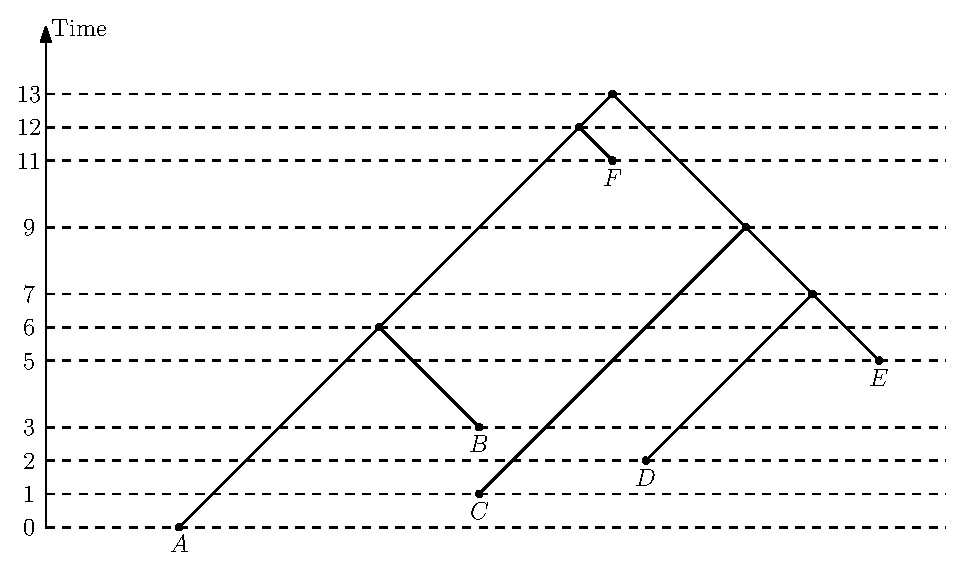
\includegraphics[width=0.7\textwidth]{timeTree.eps}
\caption{Time-tree on $6$ leaves.
Time is measured by non-negative real numbers.
If all times are integers, the tree is a discrete time-tree.}
\label{timeTree.eps}
\end{figure}

Although Markov chain Monte Carlo (MCMC) is guaranteed to sample from the true posterior given an infinite run time, it is important to understand mixing properties of the chain, which determine sampling properties for a finite time run.
The mixing properties of phylogenetic MCMC have, in the classical unrooted case, been a major area of research from both the theoretical perspective of mixing time bounds \autocite{Mossel2005-ly,Mossel2006-fo,Stefankovic2011-hu,spade2014note} and the practical perspective of performance on real data \autocite{beiko2006searching,Ronquist2006-fv,lakner2008efficiency,Whidden2015-yi}.
This research has focused on mixing over the set of discrete phylogenetic tree graph structures, because mixing over these discrete structures is the primary obstruction to MCMC convergence.

Time-trees use different MCMC transition kernels than do classical phylogenetic trees.
The discrete component of MCMC moves between classical phylogenetic trees are typically determined by their discretization.
For example, common moves include \emph{subtree prune and regraft} (SPR) moves, which cut a subtree off and reattach it at another location, and the subset of SPR moves called \emph{nearest-neighbor interchange} ($\nni$) moves.
Classically, these are applied without reference to branch lengths.
On the other hand, the discrete component of moves between time-trees are defined also in terms of their timing information.
For example, \textcite{Hohna2008-vl} show that SPR-like moves that reattach subtrees at the same divergence time are more effective than ones that do not.
This sort of move cannot be expressed using the type of discretization used thus far in which all continuous information is lost, and so the previous work on MCMC mixing cannot be applied.

However, one can discretize time-trees in a way that does preserve some of the information.
For example, by retaining the order of internal nodes backward in time one obtains a so-called \emph{ranked tree} \autocite{Semple2003-nj}.
To make a less rough approximation of a time-tree, one can allow the time periods between nodes of the tree to take only finitely many possible values \autocite{Akerborg2008-cl}.
This results in an object we call a \emph{discrete time-tree}.
The graph built on such trees provides a discretization of the space of time-trees, which we call a \emph{discrete time-tree graph}.
\DIFaddbegin \DIFadd{By a }\emph{\DIFadd{graph}} \DIFadd{on a set of trees here and throughout the paper we mean a graph consisting of trees as vertices, with edges connecting pairs of trees that are identical after a given tree rearrangement operation }\autocite{Semple2003-nj}\DIFadd{.
This graph-theoretic terminology is convenient and has become widespread in recent years }\autocite{spade2014note, Whidden2015-yi, Gavryushkin2014-bw}\DIFadd{.
}\DIFaddend A sequence of time-trees sampled using MCMC projects to a collection of movements on a graph in which each vertex is a discrete time-tree and each edge is a discrete version of an MCMC move on time-trees.

Although inferential algorithms have applied MCMC on time-trees for over a decade, and graphs corresponding to discretizations of unrooted tree space have been studied for even longer, we are not aware of any work defining graphs from discretization of time-tree spaces or analyzing random walks thereupon.
Such a theory would provide a foundation for understanding the behavior of MCMC algorithms on time-trees, as has been done previously for graphs associated with unrooted phylogenetic trees.
Up to now, the only discretization of time-tree space is that of ranked trees \autocite{Page1991-rd,Ford2009-qi,Lambert2013-mr}, and the corresponding graphs have not been studied.

In this paper we initiate the mathematical study of discrete time-tree graphs, obtain basic geometric and graph-theoretic results,
\iftoggle{curvatureON}{
study random walks on these graphs,
}{}
and compare these results to those in the classical phylogenetic setting.
In particular, we focus on ranked trees, discrete time-trees (as defined above), and the ultrametric versions of those types of trees.
We establish size bounds for neighborhoods and diameters in these tree spaces and show how those bounds can be used to develop efficient tree search algorithms such as MCMC.
\DIFaddbegin \DIFadd{The importance of these basic geometric characteristics in phylogenetics and other areas of evolutionary biology is highlighted in }\autocite{Huber2011-uu}\DIFadd{.
}\DIFaddend \iftoggle{curvatureON}{
We study Ricci-Ollivier curvature \autocite{Ollivier2009-cj} of Markov chains on these graphs, a formalism which quantifies to what extent random walking brings unit balls together.
This formalism has recently been applied to Markov chains on graphs of classical phylogenetic trees \autocite{Whidden2015-es}.
}


\section{Technical introduction}
\iftoggle{curvatureON}{
\subsection{Discrete time-trees}
}{}

Throughout the paper by a (phylogenetic) \emph{tree} we mean a rooted binary tree with designated leaves, that is, an undirected acyclic graph with the following properties:
(1) all nodes have degree $1$, $2$, or $3$; (2) there exists exactly one node of degree $2$, this node is called the \emph{root} of the tree; (3) all nodes of degree $1$ are labeled by distinct identifiers, these nodes are called \emph{leaves} or \emph{taxa} (singular \emph{taxon}).
The \emph{parent} of a node $x$ in a tree is the unique node $y$ that is both adjacent to $x$ and closer to the root of the tree than $x$.
Every node of a tree has a parent except for the root, and is called the \emph{child} of that parent.

We fix the number of leaves of the trees and denote this number by $n$ throughout the paper.
We also assume that each tree with $n$ leaves uses the same fixed set of $n$ \DIFdelbegin \DIFdel{constants }\DIFdelend \DIFaddbegin \DIFadd{labels }\DIFaddend to mark the leaves.
Hence, we say that two trees are \DIFdelbegin \DIFdel{isomorphic }\DIFdelend \DIFaddbegin \emph{\DIFadd{isomorphic}} \DIFaddend if they are isomorphic as graphs and the isomorphism maps leaves marked by the same \DIFdelbegin \DIFdel{constant }\DIFdelend \DIFaddbegin \DIFadd{label }\DIFaddend to each other.
We \DIFdelbegin \DIFdel{identify isomorphic trees}\DIFdelend \DIFaddbegin \DIFadd{do not distinguish between isomorphic trees, i.e.\ we }\emph{\DIFadd{identify}} \DIFadd{them}\DIFaddend .

By a \emph{time-tree} (Figure~\ref{timeTree.eps}) we mean a phylogenetic tree with an absolute time associated with every node of the tree so that the time strictly increases along every path from a leaf to the root: for internal nodes the time is interpreted as (typically estimated) divergence time and for leaves it is the (typically known) sampling time.
By ``absolute'' we clarify that these are not relative times, but rather actual times that can be put on a calendar.
We assume that time progresses backward, from the leaves to the root.

A \emph{discrete time-tree} is a tree such that all its nodes are assigned distinct times from the set of non-negative integers and every node has a smaller time than its parent (Figure~\ref{timeTree.eps}).
Note that this implies that for every pair of nodes $x,y$ if the shortest path from the root to $x$ passes through $y$ then the time of $y$ is greater than the time of $x$.
Each node is associated with a type of event: internal nodes represent divergence events, while leaf nodes represent the sampling of new taxa.
The \emph{rank} of a node is the number of nodes in the tree with strictly smaller time.
We say that a pair of nodes $x,y$ of a discrete time-tree is an \emph{event interval} if there exists no node $z$ such that the time of $z$ is between the time of $x$ and $y$.
\DIFaddbegin \DIFadd{Hence, an event interval is an interval between two divergence events, a taxon and a divergence event, or two taxa.
Note that taxon events can be younger than divergence nodes, i.e.\ when the sampling time precedes divergence events on the tree.
}\DIFaddend The difference between the times of $x$ and $y$ is called the \emph{length} of the interval $x,y$.
We identify two discrete time-trees if they are isomorphic as trees and the isomorphism preserves ranks of the nodes as well as event interval lengths.
\DIFdelbegin \footnote{\DIFdel{Hence, an event interval is an interval between two divergence events, a taxon and a divergence event, or two taxa.
Note that taxon events can be younger than divergence nodes, i.e.\ when the sampling time precedes divergence events on the tree.}}
%DIFAUXCMD
\addtocounter{footnote}{-1}%DIFAUXCMD
\DIFdelend 

We are now ready to introduce a hierarchy of discrete time-trees.
\DIFdelbegin %DIFDELCMD < 

%DIFDELCMD < %%%
\DIFdelend At the bottom level of our hierarchy is the well-known $\nni$ graph, which does not have timing information.
$\nni$ is a graph with the vertices being all trees on $n$ leaves.
Two trees $T$ and $R$ are adjacent in $\nni$ if there exists an edge $e$ in $T$ and an edge $f$ in $R$ such that both edges are not adjacent to a leaf and the graph obtained from $T$ by shrinking $e$ to a vertex is isomorphic to the graph obtained from $R$ by shrinking $f$.
We denote this graph by $\dtt_0$\DIFaddbegin \DIFadd{, where $\dtt$ stands for ``discrete time-trees''}\DIFaddend .

\begin{figure}[ht]
\centering
\DIFdelbeginFL %DIFDELCMD < 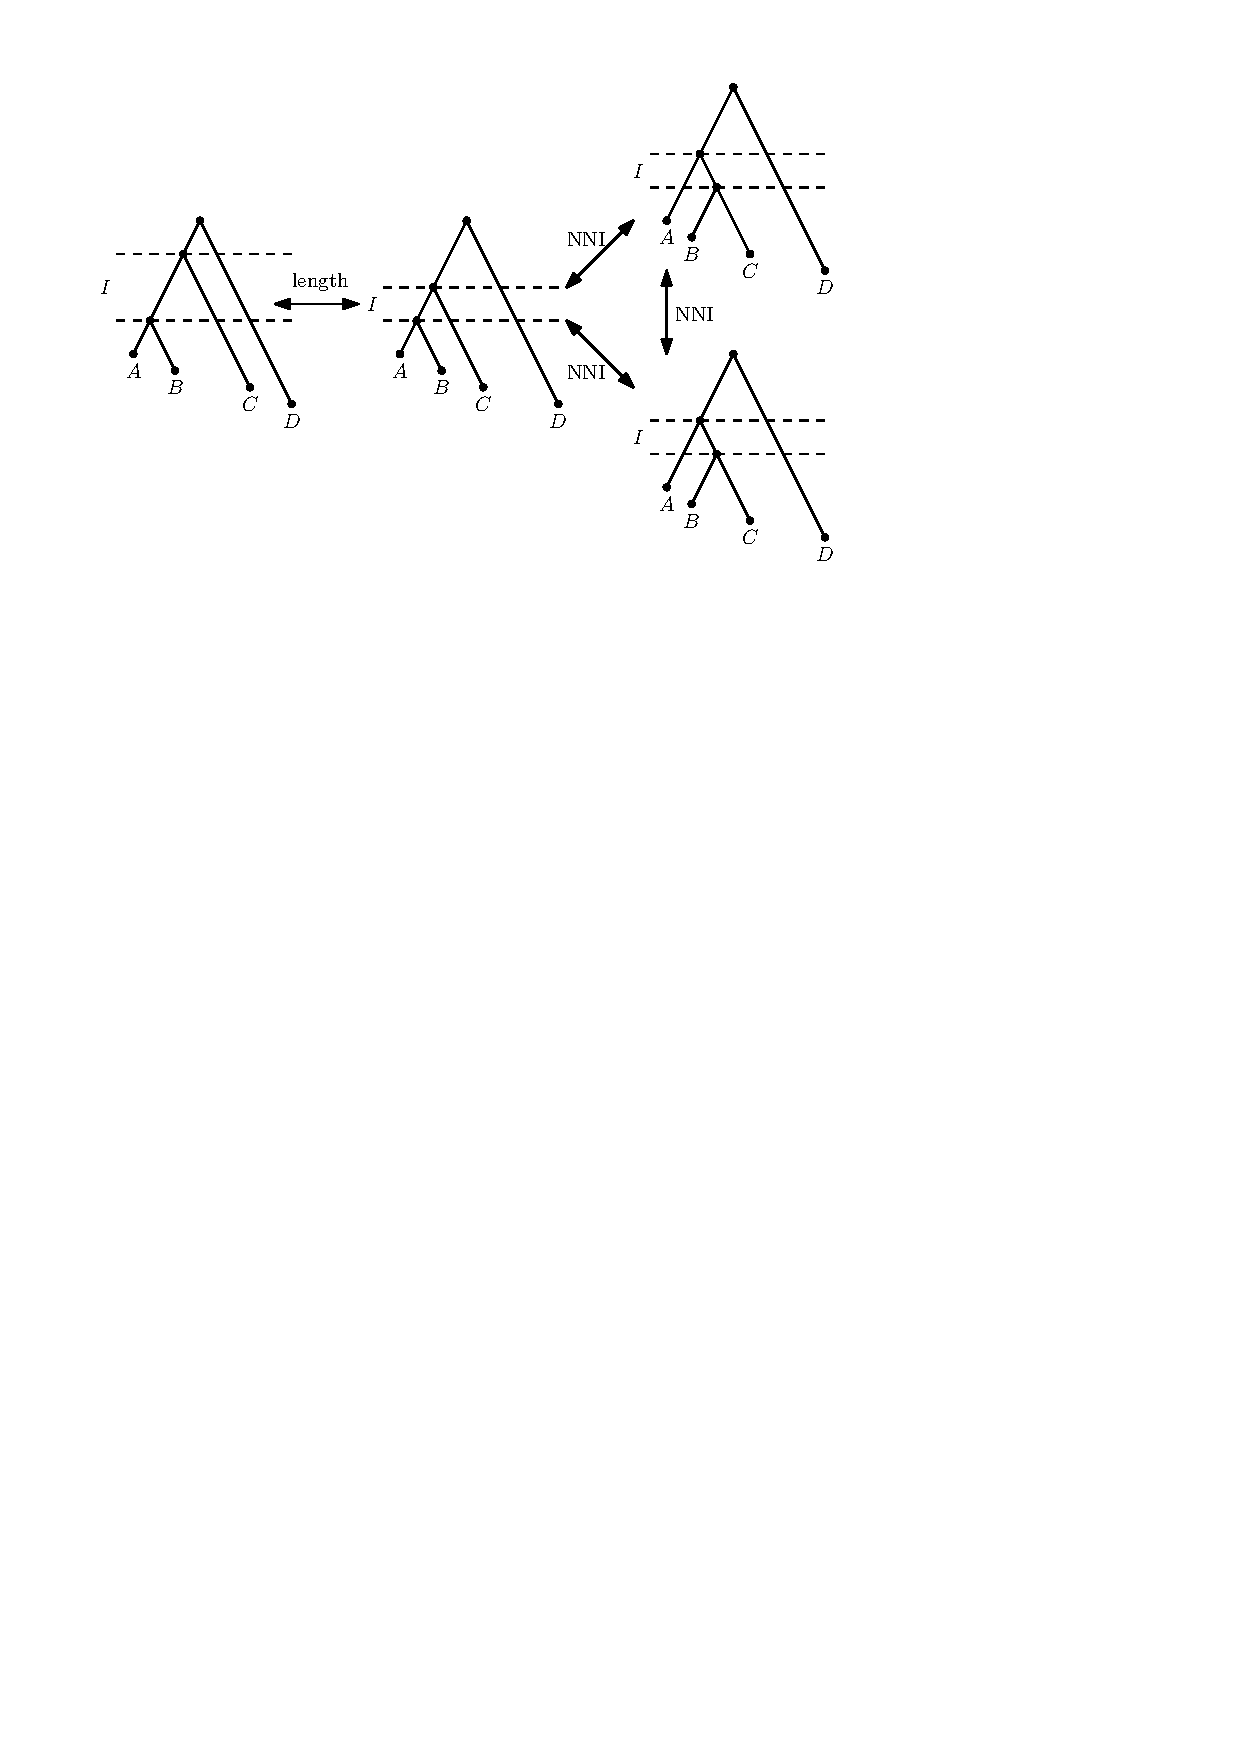
\includegraphics[width=0.8\textwidth]{DtT.pdf}
%DIFDELCMD < %%%
\DIFdelendFL \DIFaddbeginFL 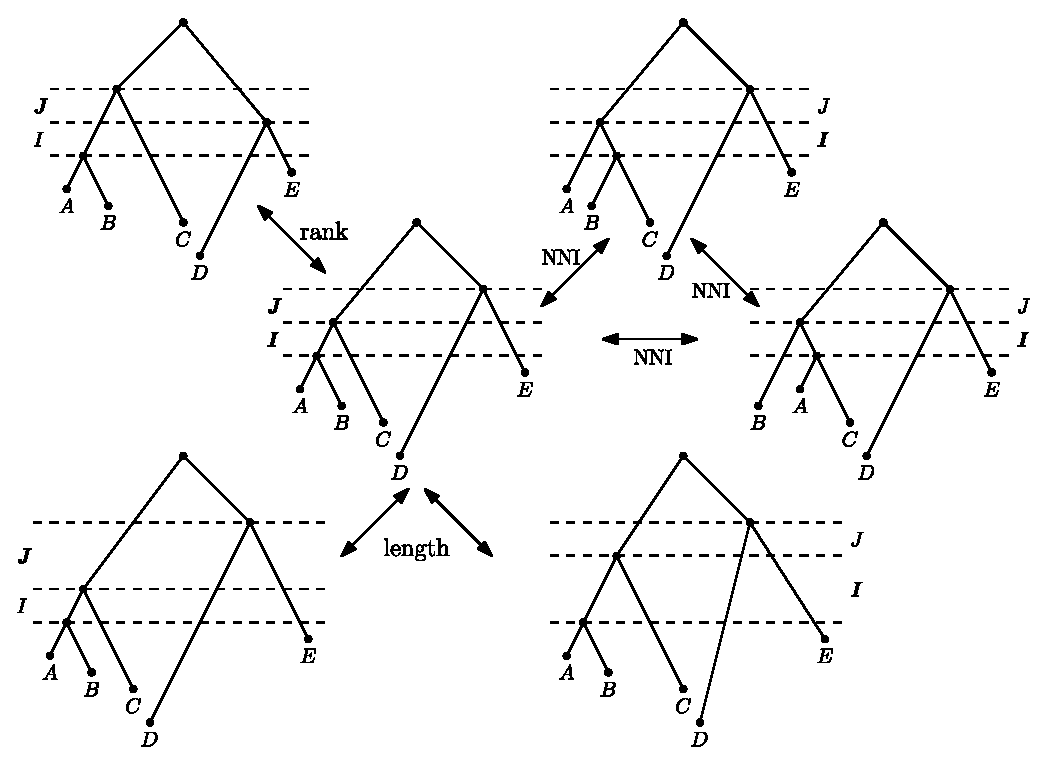
\includegraphics[width=0.8\textwidth]{DtT_with_rank_move_short_both_intervals}
%DIF > 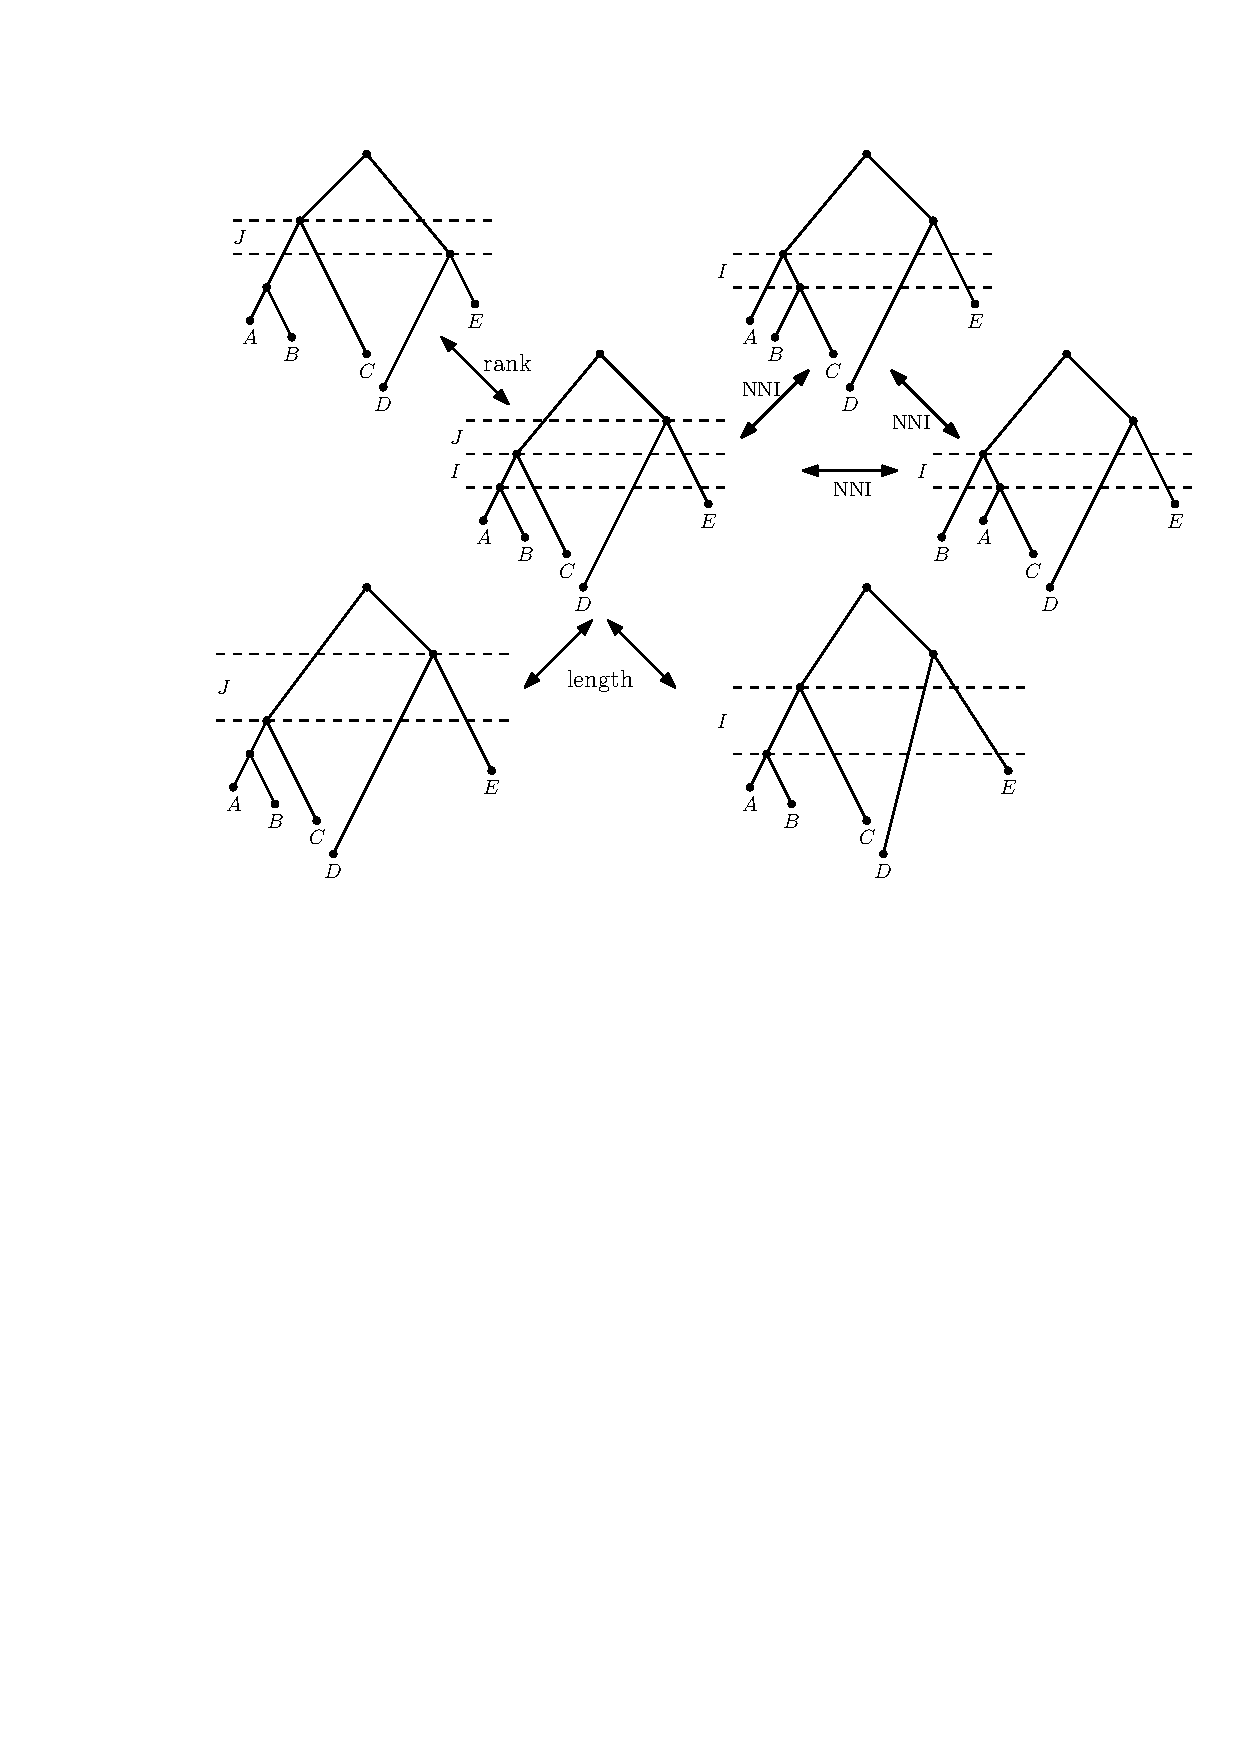
\includegraphics[width=0.8\textwidth]{DtT_with_rank_move_short}
\DIFaddendFL \caption{All possible moves performed on \DIFdelbeginFL \DIFdelFL{interval }\DIFdelendFL \DIFaddbeginFL \DIFaddFL{intervals }\DIFaddendFL $I$ \DIFaddbeginFL \DIFaddFL{and $J$}\DIFaddendFL .
Assuming that the length of every event interval is either $1$ or $2$, the outer trees are all possible neighbors in $\dtt$ of the tree in the middle \DIFdelbeginFL \DIFdelFL{corresponding to }\DIFdelendFL \DIFaddbeginFL \DIFaddFL{obtained by moves performed on intervals $I$ and $J$.
The trees on the right are obtained by moves performed on }\DIFaddendFL interval $I$ \DIFaddbeginFL \DIFaddFL{and those on the left on $J$}\DIFaddendFL .}
\label{DtT.pdf}
\end{figure}

The following graph $\dtt_m$ forms the level $m > 0$ of the hierarchy.
The set of vertices of the graph is the set of all discrete time-trees on $n$ leaves such that every event interval has its length not greater than $m$.
Two trees $T$ and $R$ are adjacent in $\dtt_m$ if $R$ can be obtained from $T$ by one of three operations: a \emph{length move performed on interval} $I$, \emph{swapping the rank of two nodes $x$ and $y$ \DIFaddbegin \DIFadd{on interval}\DIFaddend } \DIFaddbegin \DIFadd{$I$ }\DIFaddend or an \emph{$\nni$ move performed on interval $I$} (Figure~\ref{DtT.pdf}).
A length move changes the length of $I$ by 1.
Swapping the rank of two nodes \DIFdelbegin \DIFdel{$x$ and $y$ swaps their times }\DIFdelend \DIFaddbegin \DIFadd{swaps the times of the nodes; such a swap is only possible when the nodes bound an event interval $I$ of length $1$}\DIFaddend .
$R$ can be obtained from $T$ by an $\nni$ move if there exist event intervals \DIFdelbegin \DIFdel{$I$ and $J$ }\DIFdelend \DIFaddbegin \DIFadd{$I_T$ and $I_R$ }\DIFaddend of length $1$ in $T$ and $R$, respectively, such that the graphs obtained by shrinking \DIFdelbegin \DIFdel{$I$ and $J$ }\DIFdelend \DIFaddbegin \DIFadd{$I_T$ and $I_R$ }\DIFaddend to vertices are isomorphic and the isomorphism preserves the lengths of the event intervals.
In other words, by going from one tree to an adjacent tree in the $\dtt_m$ graph we can either change the length of one event interval by one unit, swap the rank of two nodes \DIFaddbegin \DIFadd{bounding an event interval of minimal length}\DIFaddend , or send the length of an event interval of minimal length down to zero and then resolve the multifurcation to either of the two possible trees.
In the latter case, the new interval is of minimal length.
See Figure~\ref{dts_neighbors.pdf} for an example of the full variety of possible moves.

\begin{figure}[ht]
\centering
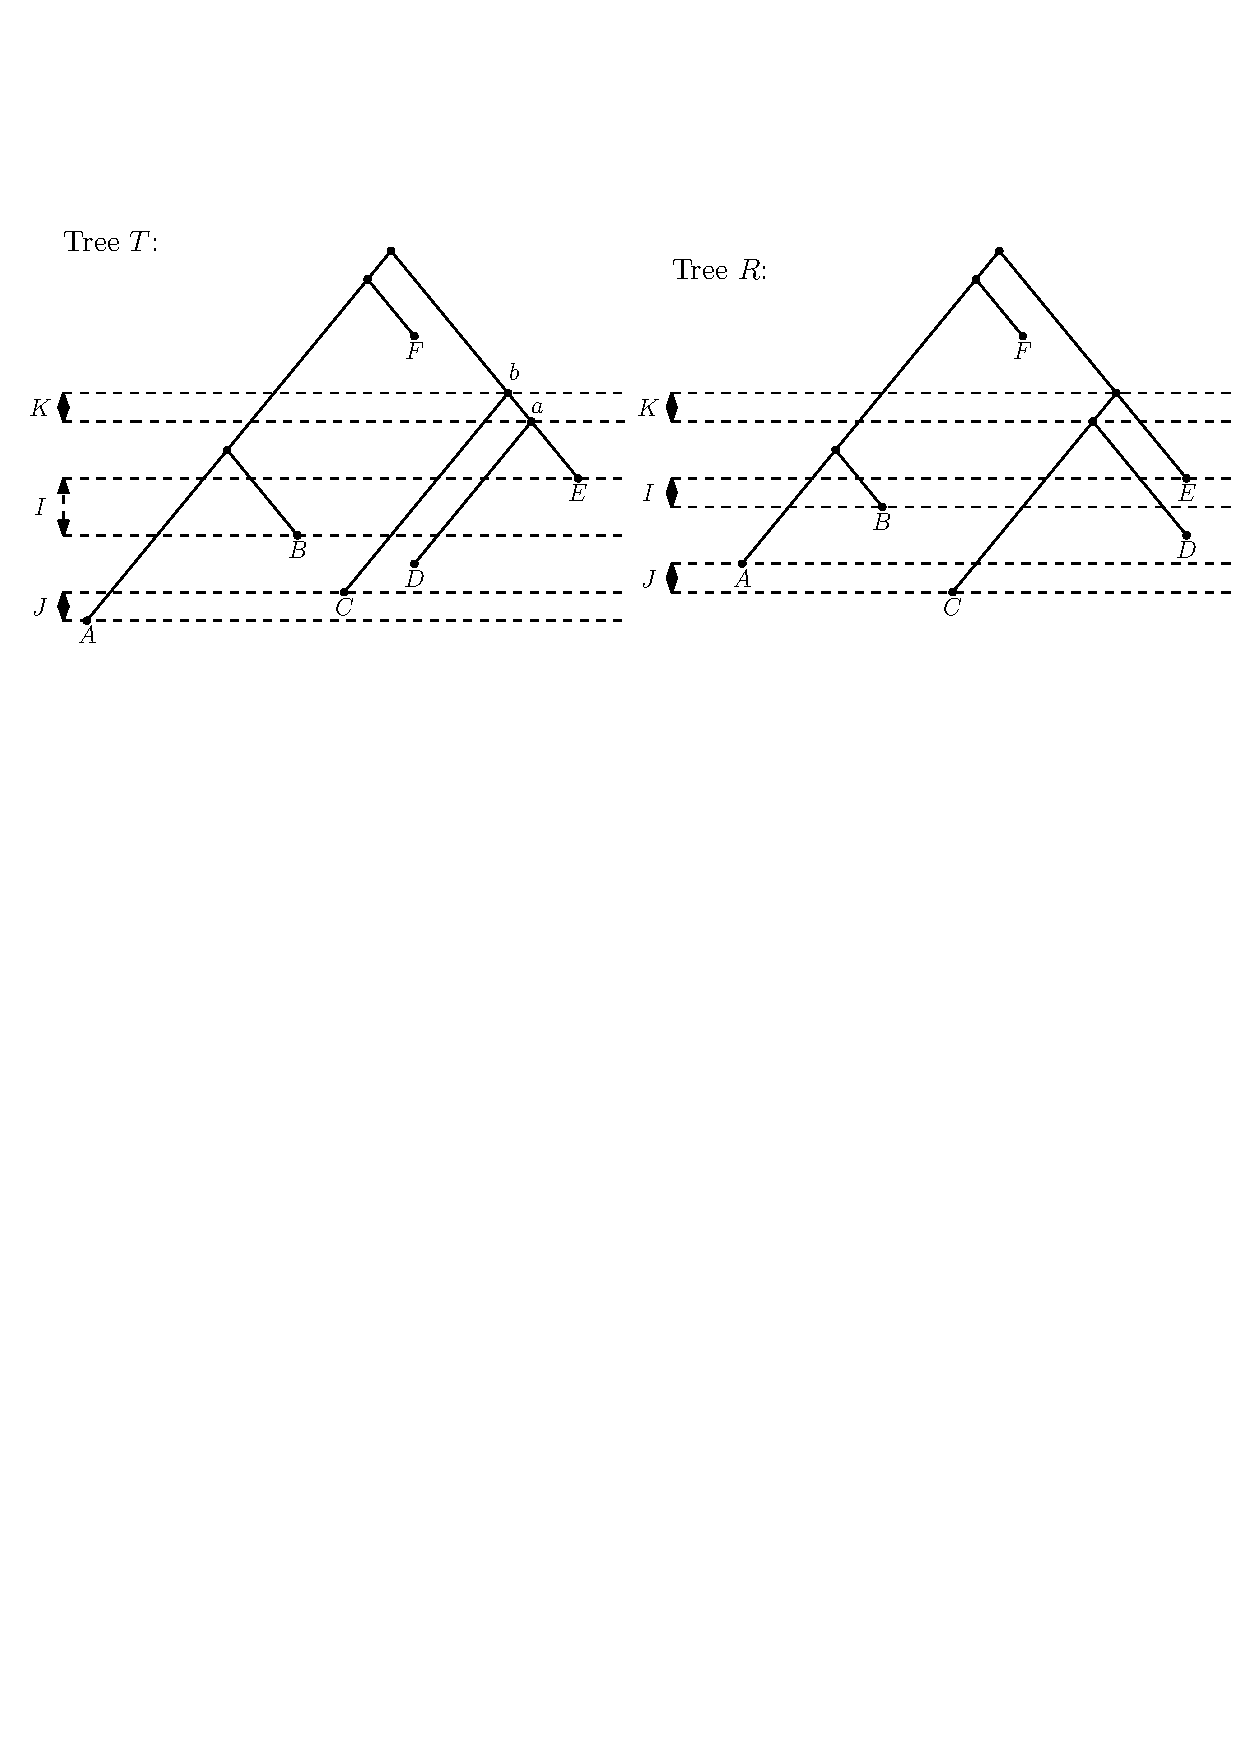
\includegraphics[width=\textwidth]{dts_neighbors.pdf}
\caption{Trees $T$ and $R$ are at $\dtt_2$ distance $3$.
To move from $T$ to $R$ in $\dtt_2$, one must decrease the length of interval $I$, swap the ranks of nodes $A$ and $C$ bounding interval $J$, and perform an $\nni$ move on interval $K$, resolving nodes $C$ and $D$.}
\label{dts_neighbors.pdf}
\end{figure}

Note that $\dtt_0$ can be obtained from $\dtt_1$ by ``forgetting'' ranks and $\dtt_1$---from $\dtt_m$ by forgetting lengths.
In general, the graph structure for $m > 1$ can be understood by considering all \DIFdelbegin \DIFdel{diagrams as }\DIFdelend \DIFaddbegin \DIFadd{four-tree diagrams as the four trees on the right }\DIFaddend in Figure~\ref{DtT.pdf} and introducing an extra layer of nodes in every tail adjacent to the \DIFdelbegin \DIFdel{triangle on the right of the diagram}\DIFdelend \DIFaddbegin \DIFadd{$\nni$ triangle}\DIFaddend .

This hierarchy can be seen as a set of discrete refinements of the full space of phylogenetic time-trees, where event intervals can take an arbitrary real value.
Indeed, if we \DIFdelbegin \DIFdel{consider
$\tau$-space}\footnote{\DIFdel{Conveniently, the discrete versions of $\tau$- and $\mathrm t$-space from }%DIFDELCMD < \autocite{Gavryushkin2014-bw} %%%
\DIFdel{coincide.}}
%DIFAUXCMD
\addtocounter{footnote}{-1}%DIFAUXCMD
\DIFdel{defined by \textcite{Gavryushkin2014-bw} and allow the real-valued parameters (length }\DIFdelend \DIFaddbegin \DIFadd{allow the lengths }\DIFaddend of event intervals \DIFdelbegin \DIFdel{) to take only $m$ possible values from $1,\ldots,m$ }\DIFdelend \DIFaddbegin \DIFadd{to take every possible non-negative real value and impose the Euclidean metric on trees with the same ranked topology, }\DIFaddend then we get \DIFdelbegin \DIFdel{$\dtt_m$}\DIFdelend \DIFaddbegin \DIFadd{the $\tau$-space introduced by \textcite{Gavryushkin2014-bw}}\DIFaddend .
In this case, \DIFdelbegin \DIFdel{$\dtt_0$ }\DIFdelend \DIFaddbegin \DIFadd{$\dtt_1$ }\DIFaddend is the graph with the vertices being the \DIFdelbegin \DIFdel{cubes }\DIFdelend \DIFaddbegin \DIFadd{orthants }\DIFaddend of $\tau$-space and the adjacency relation being the relation of ``have a shared facet of co-dimension $1$\DIFdelbegin \DIFdel{''}\DIFdelend \DIFaddbegin \DIFadd{.''
Similarly $\dtt_0$ is the adjacency graph on the orthants of BHV space }\autocite{Billera2001-rj}\DIFaddend .

The $\dtt_m$ graph on ultrametric trees, that is the set of trees such that each leaf has the same time, is denoted by $\dttu_m$.
The $\dtt_1$ graph is denoted by $\rnni$ and called the \emph{ranked $\nni$} graph; on ultrametric trees we will denote it $\rnniu$.
\DIFdelbegin \footnote{\DIFdel{Note that the R in $\rnni$ stands for }\emph{\DIFdel{ranked}} %DIFAUXCMD
\DIFdel{and not for rooted.}}
%DIFAUXCMD
\addtocounter{footnote}{-1}%DIFAUXCMD
\DIFdelend \DIFaddbegin \DIFadd{The $\mathrm R$ in $\rnni$ stands for }\emph{\DIFadd{ranked}} \DIFadd{and not for rooted.
}\DIFaddend We emphasize that although this is the $\rnni$ \emph{graph}, \DIFdelbegin \DIFdel{NNI }\DIFdelend \DIFaddbegin \DIFadd{$\nni$ }\DIFaddend \emph{moves} can be applied to trees in any of the spaces considered (under appropriate conditions).
For simplicity, we use the generic identifier $\dtt$ to refer to a $\dtt_m$ with an arbitrary $m > 1$.

A graph can also be seen as a metric space where the distance is given by the length of a shortest path, so we will refer to $\dtt_m$ and other graphs introduced below as both\DIFaddbegin \DIFadd{, in agreement with }\autocite{Semple2003-nj}\DIFaddend .

\iftoggle{curvatureON}{
Furthermore, as $\nni$ graph on unrooted tree topologies with $n-1$ leaves is isomorphic (as a graph) to the $\nni$ graph on rooted tree topologies with $n$ leaves, all our results on curvature immediately imply their counterparts in unrooted $\nni$ graph.
We omit from the text the exact formulations for unrooted trees, as they can be obtained in the obvious way.


\subsection{Ricci-Ollivier curvature}
A random walk on a metric space is defined by its proposal mechanism, which is a functional $m$ that maps points of the space to the set of measures on this space \autocite[see][]{Ollivier2009-cj}.
In other words, for every point $v$ in the space, $m(v,w)$, which we denote by $m_v(w)$, is the probability of the random walk moving from $v$ to $w$ in one step.
Given a metric space $(V,d)$, a \emph{coupling} $\mu$ between two measures $\mu_1$ and $\mu_2$ on $V$ is a probability measure on the set of pairs of points $V \times V$ that is $\mu_1$ after marginalizing over the second component, and $\mu_2$ after marginalizing over the first component, that is, $\sum\limits_{y \in V}\mu(x,y) = \mu_1(x)$ and $\sum\limits_{y \in V}\mu(y,x) = \mu_2(x)$ for all $x \in V$.
A coupling can be seen as a scenario of transforming the measure $\mu_1$ on $V$ to $\mu_2$ by looking at $\mu(x,y)$ as the probability mass that has to be moved from $x$ to $y$ under the scenario.

Using these notations, we define the \emph{work} $\W_\mu$ needed to be done to transform $\mu_1$ to $\mu_2$ via coupling $\mu$ by setting
\[
\W_\mu(\mu_1,\mu_2) = \sum\limits_{x,y\in V}\mu(x,y) d(x,y).
\]
Let $\M$ be the set of all couplings between measures $\mu_1$ and $\mu_2$.
Then the \emph{earth mover's distance} $W$ between $\mu_1$ and $\mu_2$ is defined to be $W(\mu_1,\mu_2) = \inf\limits_{\mu\in\M}\W_\mu(\mu_1,\mu_2)$.

We are now ready to introduce two curvature notions that we are studying in this paper.
Let $m$ be a random walk on a metric space $(V,d)$.
Then the \emph{coarse Ricci-Ollivier curvature} between two points $x$ and $y$ from $V$ with the random walk $m$ is
\[
\kappa(m;x,y) = 1 - \frac{W(m_x,m_y)}{d(x,y)}
\]

Another important notion of this paper is that of asymptotic curvature.
The following random walk $m$ is called a \emph{uniform $p$-lazy random walk} on a metric space $(V,d)$:
\[
m_x(y) =
\begin{cases}
1-p			& \mbox{ if } x=y \\
0   			& \mbox{ if } d(x,y) > 1 \\
\dfrac{p}{|N(x)|}	& \mbox{ if } d(x,y) = 1 \\
\end{cases}
\]
where $x,y \in V$ and $N(x) = \{y \mid d(x,y) = 1\}$.

We follow \textcite{Loisel2014-gu} and define \emph{asymptotic Ricci-Ollivier curvature} $\ric$ between points $x,y$ from a metric space with uniform $p$-lazy random walk $m$ by
\[
\ric(x,y) = \lim_{p\to0} \frac{\kappa(m;x,y)}{p}
\]

One of the central properties of Ricci-Ollivier curvature is that the curvature is a local property \autocite{Ollivier2009-cj}.
For finite metric spaces that means that for all distinct $u$ and $v$,
\[
\inf\{\kappa(m;x,y)\mid d(x,y) = 1\} \leq \kappa(m;u,v).
\]
Hence, we define the \emph{coarse Ricci-Ollivier curvature of a metric space} with a random walk $m$ to be $\inf\{\kappa(m;x,y)\mid d(x,y) = 1\}$ and the \emph{asymptotic Ricci-Ollivier curvature of a metric space} to be $\inf\{\ric(x,y)\mid d(x,y) = 1\}$.
}{}


\section{Geometry and complexity of discrete time-trees}

We begin by considering the shortest path distance on the graphs.
It is well-known that computing distances is NP-hard in $\nni$ \autocite{Dasgupta2000-xa}.
Hence the following question is natural.

\begin{problem}
\label{problemComplexity}
What is the complexity of computing the distance between two discrete time-trees?
\end{problem}

Although this problem remains open, we make progress towards the solution by establishing several geometric and algorithmic properties of these graphs.
First, we demonstrate in the following example that even for caterpillar trees \DIFdelbegin \footnote{\DIFdel{Caterpillar trees, sometimes called ladder trees, have all leaves connected to a single path from the root.}}
%DIFAUXCMD
\addtocounter{footnote}{-1}%DIFAUXCMD
\DIFdelend the complexity cannot be derived from that of $\nni$ distance.
\DIFaddbegin \DIFadd{A }\emph{\DIFadd{caterpillar tree}} \DIFadd{(sometimes called a }\emph{\DIFadd{ladder tree}}\DIFadd{) has all leaves connected to a single path from the root.
A }\emph{\DIFadd{cherry}} \DIFadd{is a pair of taxa adjacent to a common internal node in the tree.
}\DIFaddend 

\begin{example}
\DIFaddbegin \label{ex_caterpillars}
\DIFaddend Let $T$ be the ultrametric caterpillar tree denoted $((((((1, 2), 3), 4), 5), 6), 7)$ in Newick notation \autocite{felsenstein1990newick} and $R$ be the ultrametric tree $((((((1, 4), 5), 6), 2), 3), 7)$.
Then a shortest $\nni$ path is given by first making a cherry $(2,3)$, then moving the cherry up to the split $1456 \mid 7$, and then resolving the cherry back.
In $\rnniu$ this path is not shortest, and one shortest path moves the parents of $2$ and $3$ up independently.

\begin{figure}[ht]
\centering
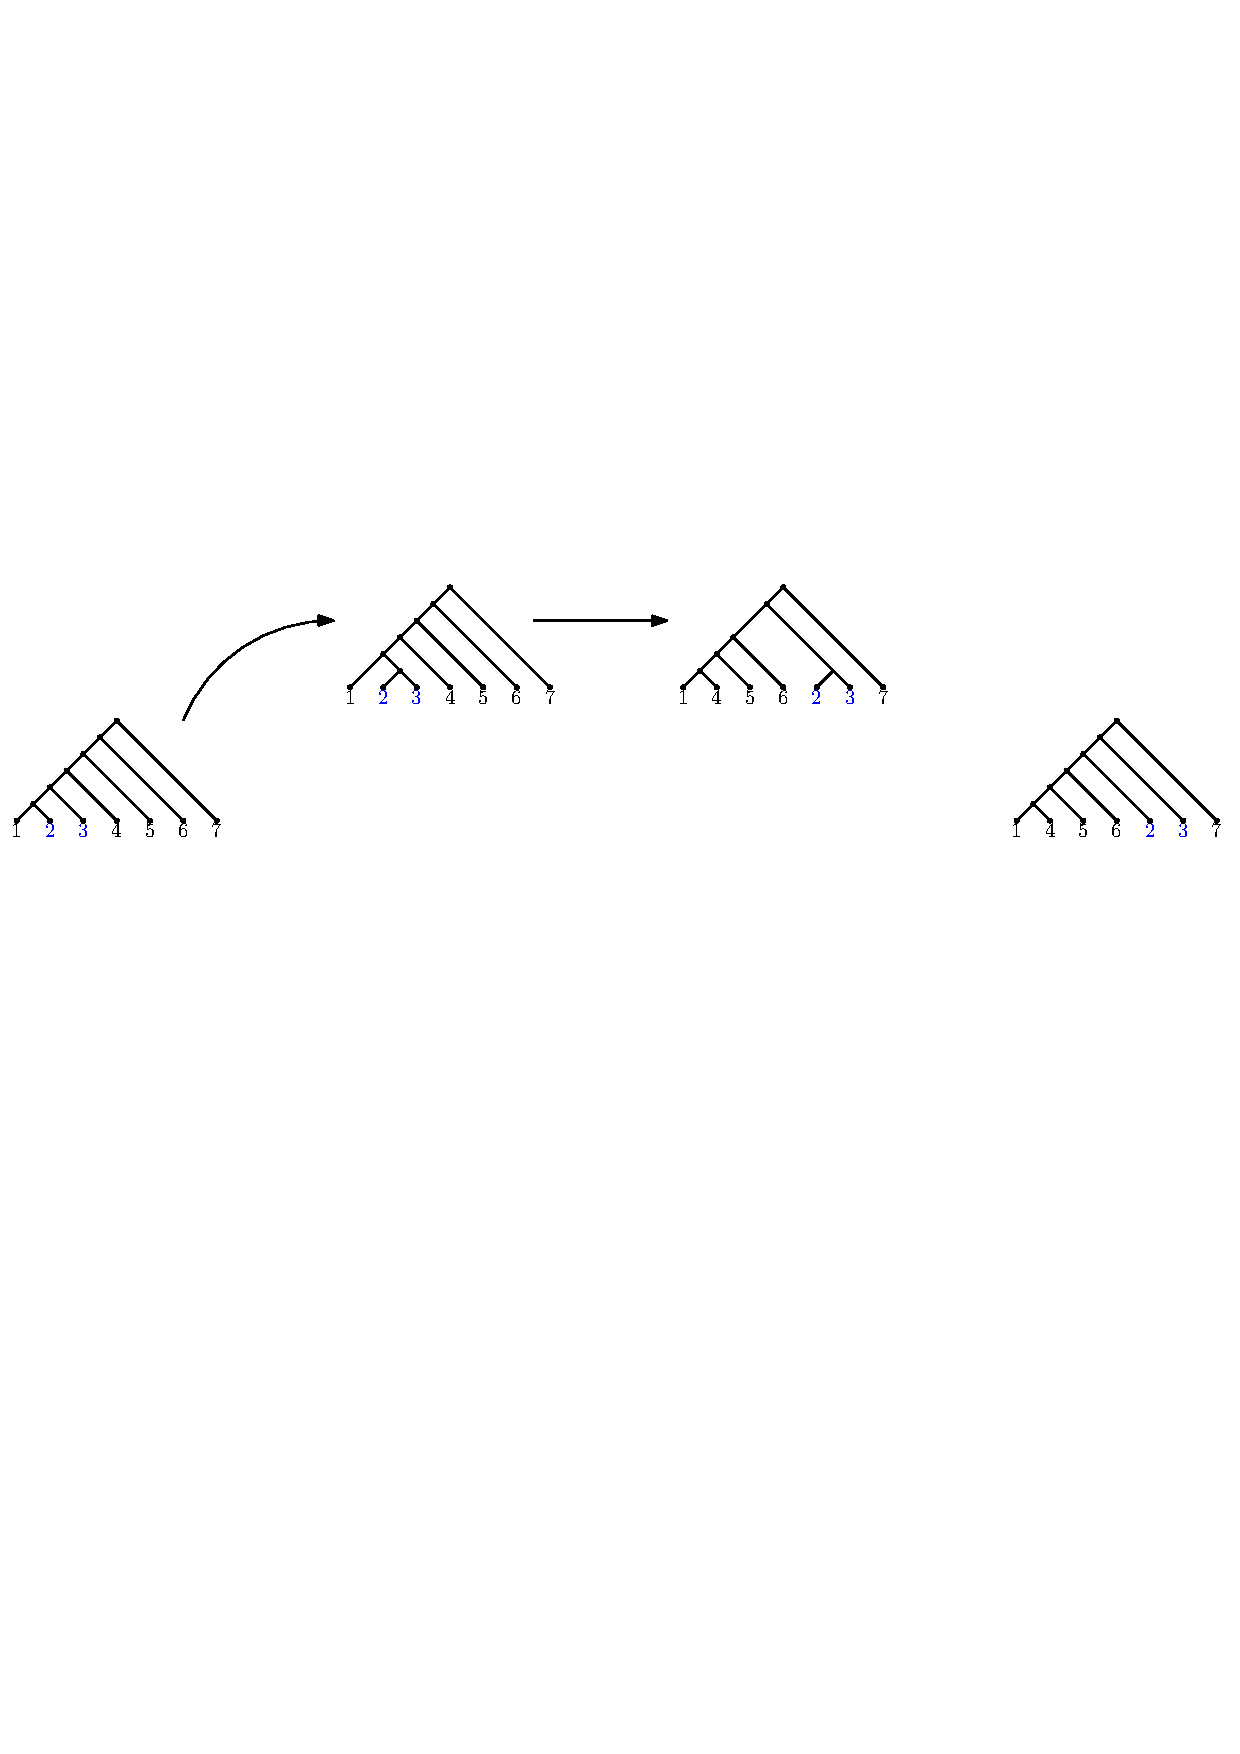
\includegraphics[width=\textwidth]{NNI_VS_rNNI.pdf}
\caption{Shortest paths in $\nni$ may not be shortest in $\rnni$.}
\label{NNI_VS_rNNI.pdf}
\end{figure}
\end{example}

\DIFdelbegin \DIFdel{This example }\DIFdelend \DIFaddbegin \DIFadd{A set of trees $A$ is called }\emph{\DIFadd{convex}} \DIFadd{if for every pair of trees from $A$, there exists a shortest path between them such that every tree on the path belongs to $A$.
Example~\ref{ex_caterpillars} }\DIFaddend can be generalized to show that the set of trees of the form $(\ldots(1, i_2), \ldots, i_{n-1}), n)$, where $\{i_2, \ldots, i_{n-1}\} = \{2, \ldots, n-1\}$, is convex in $\dtt$ and is not convex in $\nni$.
Indeed, the example shows that if two leaves have to be moved up, they can be moved independently along a shortest path.
The generalization of this statement to an arbitrary number of leaves implies convexity in $\dtt$, while the need to group leaves in $\nni$ as in the previous example shows non-convexity in $\nni$ space.
This basic difference in the structure of the two graphs suggests that the complexity of computing the distance is likely to be different.

We proceed by establishing basic geometric properties of discrete time-trees.


\subsection{Sizes of neighborhoods}

We first bound the number of trees in each graph.
As expected, times greatly expand the size of the graphs.

\begin{lemma}[see \autocite{Semple2003-nj}]
\label{spaceSizes}
Let $|V|$ be the number of vertices in the graph, then $|V|$ is equal to
\begin{align*}
& \frac{(n-1)!\,n!\,n!\,m^{n-1}}{2^{n-1}}	& \mbox{in $\dtt_m$,}
&&& \frac{(n-1)!\,n!\,m^{n-1}}{2^{n-1}}		& \mbox{in $\dttu_m$,}\\
& \frac{(n-1)!\,n!\,n!}{2^{n-1}}		& \mbox{in $\rnni$,}
&&& \frac{(n-1)!\,n!\,}{2^{n-1}}		& \mbox{in $\rnniu$,}\\
& (2n - 3)!!					& \mbox{in $\nni$.}
\end{align*}
\end{lemma}

\proof
The proof for $\nni$ can be found in \autocite{Semple2003-nj}.
The rest follow using similar arguments.
\endproof

We continue by tightly bounding the sizes of $1$-neighborhoods of various discretizations of the space of time-trees.
Each has a $1$-neighborhood size that is linear in $n$ allowing for efficient local traversal and enumeration\DIFaddbegin \DIFadd{, }\DIFaddend a property of importance for phylogenetic algorithms, e.g.\ tree proposals in MCMC.

\iftoggle{curvatureON}{
We will use these bounds to estimate the curvature of various random walks later in the paper.
}{}

\begin{lemma}
\label{neighBound}
Let $T$ be a tree on $n$ leaves and $\deg(T)$---the number of trees adjacent to $T$.
Then
\begin{align*}
& 2(n-1) \leq \deg(T) \leq 5n-6	& \mbox{in $\dtt$,}
&&& n-1 \leq \deg(T) \leq 3n-5	& \mbox{in $\dttu$,}\\
& n-1\leq \deg(T) \leq3n-4 	& \mbox{in $\rnni$,}
&&& n-1 \leq \deg(T) \leq 2n-4 	& \mbox{in $\rnniu$,}\\
& \deg(T) = 2n-4 		& \mbox{in $\nni$.}
\end{align*}
All bounds are tight.
\end{lemma}

\proof
\DIFaddbegin \DIFadd{We prove the bounds by providing exemplar trees with the specified degrees and explaining why no tree can have a greater (or lesser) degree.
Recall that $m > 1$ is the maximal possible length of an event interval in a tree from $\dtt$.
}\DIFaddend The lower bound in $\dtt$ is attained by any tree with all event intervals being of length $m$.
\DIFdelbegin \footnote{\DIFdel{Recall that $m > 1$ is the maximal possible length of an event interval in a tree from $\dtt$.}}
%DIFAUXCMD
\addtocounter{footnote}{-1}%DIFAUXCMD
\DIFdelend In this case, $\deg(T)$ is simply the number of event intervals, since every event interval adds $1$ to the total degree of the tree.
Other trees have the same or more possible event interval changes, showing that this is a lower bound.
The upper bound is attained by a caterpillar tree with all intervals short\DIFdelbegin \DIFdel{and no divergence event}\DIFdelend \DIFaddbegin \DIFadd{, every taxon being younger than every divergence event, and both taxa in the cherry }\DIFaddend being younger than \DIFdelbegin \DIFdel{a taxon}\DIFdelend \DIFaddbegin \DIFadd{at least one other taxon, that is, a caterpillar tree with internal nodes having ranks $n, \ldots, 2(n-1)$ and the ranks of the taxa in the cherry $< n-1$}\DIFaddend .
In this case, $\deg(T)$ is bounded by the sum of the $2(n-1)$ possible interval length changes, \DIFdelbegin \DIFdel{the }\DIFdelend at most $2(n-2)$ $\nni$ neighbors, and at most $n$ rank changes that can occur between the $n$ taxa \DIFaddbegin \DIFadd{and the root of the cherry}\DIFaddend .
In total, $\deg(T) \le 2(n-1) + 2(n-2) + n = 5n-6$.
Note that this is an upper bound indeed, as each of the $2(n-2)$ intervals excluding the most recent can contribute either a rank change or $2$ $\nni$ moves.
The caterpillar tree described above maximizes the number of intervals that contribute $2$ $\nni$ moves and enables the rest of intervals to contribute a rank change.

For ultrametric trees, the number of event intervals is $n-1$, hence they add $n-1$ to the degree of the caterpillar tree from interval \DIFaddbegin \DIFadd{length }\DIFaddend changes.
The number of intervals on which an $\nni$ move is possible is $n-2$ for ultrametric trees, hence they contribute $2(n-2)$ to the degree.
In total, this gives the upper bound of $3n-5$ for ultrametric trees.

Every $\nni$ move results in two neighbors, so the equality $\deg(T) = 2(n-2)$ follows for the $\nni$ graph.
Indeed, \DIFdelbegin \DIFdel{it is not hard to see that the set of }\DIFdelend \DIFaddbegin \DIFadd{no $\nni$ move can be performed on an edge adjacent to a taxon, exactly two }\DIFaddend $\nni$ moves \DIFdelbegin \DIFdel{that only consider moving a subtree to its aunt captures the full set of }\DIFdelend \DIFaddbegin \DIFadd{can be performed on every edge between internal nodes (the number of which is $n-2$), and no two trees obtained by an }\DIFaddend $\nni$ \DIFdelbegin \DIFdel{neighbors with no duplicates.
The neighborhood size then follows because the root and its two children have no aunt}\DIFdelend \DIFaddbegin \DIFadd{move performed on different edges are identical}\DIFaddend .

The lower bound in $\rnni$ is attained by the caterpillar-tree where taxa get ranks $0, 1, 3, 5, \ldots, 2n-3$ and internal nodes get ranks $2, 4, 6, \ldots, 2n-2$.
In other words, the divergence events alternate with the taxa in the ranked topology of the tree so that if we parse the tree from the present to the past, we meet the nodes in the following order: taxon, taxon, coalescence, taxon, coalescence, taxon, coalescence, and so on.
In this case, intervals bounded by a taxon from below add nothing to the degree of the tree and intervals bounded from below by an internal node add one each, hence $n-1$ in total.
The upper bound for both $\rnni$ and $\rnniu$ is obtained in the same way as for $\dtt$.

For the lower bound in $\rnniu$, we note that the oldest event interval (the one adjacent to the root) necessarily contributes $2$ to the degree.
Hence the lower bound can be reached by a tree such that no other interval contributes more than 1.
The degree of such a tree is $n-1$ in $\rnniu$.
\endproof

Lemma~\ref{neighBound} gives tight bounds for the number of trees in a $1$-neighborhood, while the following theorem gives an upper bound for the number of trees in an $r$-neighborhood.
The \DIFdelbegin \DIFdel{following theorem bounds the sizes of neighborhoods.
The best known }\DIFdelend \DIFaddbegin \DIFadd{best known upper }\DIFaddend bound for $\nni$ that we are aware of is $3^{n-2} 2^{4r}$ \autocite{li1996some}.
We obtain a smaller bound for $\rnniu$ and, hence, improve the result for $\nni$ as well.

\begin{theorem}
\label{neighSizeTh}
The number of trees within distance $r$ from any given tree is at most
\begin{align*}
& 3^{n+2r-1}	& \mbox{in $\rnniu$,}
&&& 3^{2n+2r-1}	& \mbox{in $\rnni$,}\\
& 4^{n+2r-1}	& \mbox{in $\dtt$,}
&&& 4^{2n+2r-1}	& \mbox{in $\dttu$.}
\end{align*}
\end{theorem}

\proof
We describe the proof in detail for $\rnniu$ \DIFdelbegin \DIFdel{, and include proof sketches }\DIFdelend \DIFaddbegin \DIFadd{and then explain how to modify the proof }\DIFaddend for the other three graphs\DIFdelbegin \DIFdel{in Section~6.\ Appendix}\DIFdelend .
The proof employs the technique by \textcite{Sleator1992-bp} for counting paths in a graph \DIFdelbegin \DIFdel{: we }\DIFdelend \DIFaddbegin \DIFadd{using a }\emph{\DIFadd{graph grammar}}\DIFadd{.
A graph grammar is a method of encoding each possible graph as a finite set of productions (described more formally below).
Given the grammar, the number of possible productions to the power of the encoding length for a given neighborhood radius gives a simple upper bound on the number of trees in a neighborhood.
Specifically, Theorem~2.3 from }\autocite{Sleator1992-bp}\DIFadd{, adapted to trees, states the following:
}

 \begin{itemize} 
\item[] \DIFadd{Let $T$ be a tree with $h$ nodes, including all internal nodes and taxa, $\Gamma$ be a graph grammar, $d$ be the number of vertices in left sides of $\Gamma$, and $k$ be the maximum number of nodes in any right side of a production of $\Gamma$.
Let $R(T, \Gamma, r)$ be the set of graphs obtainable from $T$ by derivations in $\Gamma$ of length at most $r$.
Then $|R(T, \Gamma, r)| \leq (d + 1)^{h+k\cdot r}$.
} \end{itemize} 

\DIFadd{We }\DIFaddend first apply Theorem~2.3 from \autocite{Sleator1992-bp} and then improve the bound using specific properties of the $\rnniu$ graph.
We note that since our trees are ranked trees, they possess additional structure (ranking) on top of the tree graph structure, hence we will be applying the same style of argument as in \autocite{Sleator1992-bp} but to a somewhat different structure.

We \DIFdelbegin \DIFdel{first need to }\DIFdelend \DIFaddbegin \DIFadd{now }\DIFaddend introduce the \emph{graph grammar} for $\rnniu$.
\DIFdelbegin \DIFdel{Recall that a }\DIFdelend \DIFaddbegin \DIFadd{Since we will apply the graph grammar to modify trees, we use the graph-theoretic terminology here and recall that a tree is a graph.
A }\DIFaddend graph grammar consists of a finite set of productions $\{L_i \to_i R_i\}$, where $L_i$ and $R_i$ are connected undirected edge-end labeled graphs and $\to_i$ is a one-to-one map between half-edges of $L_i$ and those of $R_i$.
\DIFaddbegin \DIFadd{Here, for every edge in the tree we distinguish between its two ends and refer to them as half-edges---this is necessary to be able to substitute one subgraph by another in a unique way by connecting corresponding half-edges---as in }\autocite{Sleator1992-bp}\DIFadd{.
}\DIFaddend The productions are then applied to the starting tree $T$ to derive all possible trees at $\rnniu$ distance up to $r$ from $T$.
\DIFaddbegin \DIFadd{By a }\emph{\DIFadd{running tree at stage $s$}} \DIFadd{we mean the tree obtained after $s$ applications of the production rules in the derivation.
}\DIFaddend A production is said to be \emph{ready} at a stage $s$ of the derivation if the running tree at stage $s$ has a subgraph isomorphic to the left side $L_i$ of the production.
\DIFdelbegin \footnote{\DIFdel{By a }\emph{\DIFdel{running tree at stage $s$}} %DIFAUXCMD
\DIFdel{we mean the tree obtained after $s$ applications of the production rules in the derivation.}}
%DIFAUXCMD
\addtocounter{footnote}{-1}%DIFAUXCMD
\DIFdelend A ready production can be applied to the running tree by destroying all nodes corresponding to the left side of the production under the isomorphism and replacing them with the right side $R_i$ of the production.
The map $\to_i$ of the production then says how to reconnect the right side of the production to the half-edges of the running tree that were created after the destruction.
The obtained tree is the new running tree for the next stage $s+1$ of the derivation.
\DIFdelbegin %DIFDELCMD < 

%DIFDELCMD < %%%
\DIFdel{Given the grammar, the number of possible productions to the power of the encoding length for a given neighborhood radius gives a simple upper bound on the number of trees in a neighborhood.
}\DIFdelend See \autocite{Sleator1992-bp} for precise definitions and details.

The graph grammar for $\rnniu$ is the grammar $\Gamma$ shown on Figure~\ref{grammar_rNNIu.pdf}.
Note that the definition of a graph grammar requires the left sides $L_i$ to be connected and we have a disconnected left side in the third production.
We can adapt our graph grammar to fit this requirement by noting that the nodes on the left side of the production must be of consecutive ranks, so we consider those nodes as being adjacent via a second type of adjacency relation by declaring nodes with consecutive ranks to be adjacent.
This second type of relation is in addition to the first type of adjacency relation given by the branches of the tree.
Furthermore, this second type of adjacency allows us to avoid considering two separate moves for the left and right sister nodes.
Indeed, the half-edge labels order the edges to make the distinction between left and right, however since our nodes are ordered via ranking, this ordering of edges is irrelevant.
We will further exploit this important property below, where we improve the bound obtained directly from grammar $\Gamma$.

\begin{figure}
\centering
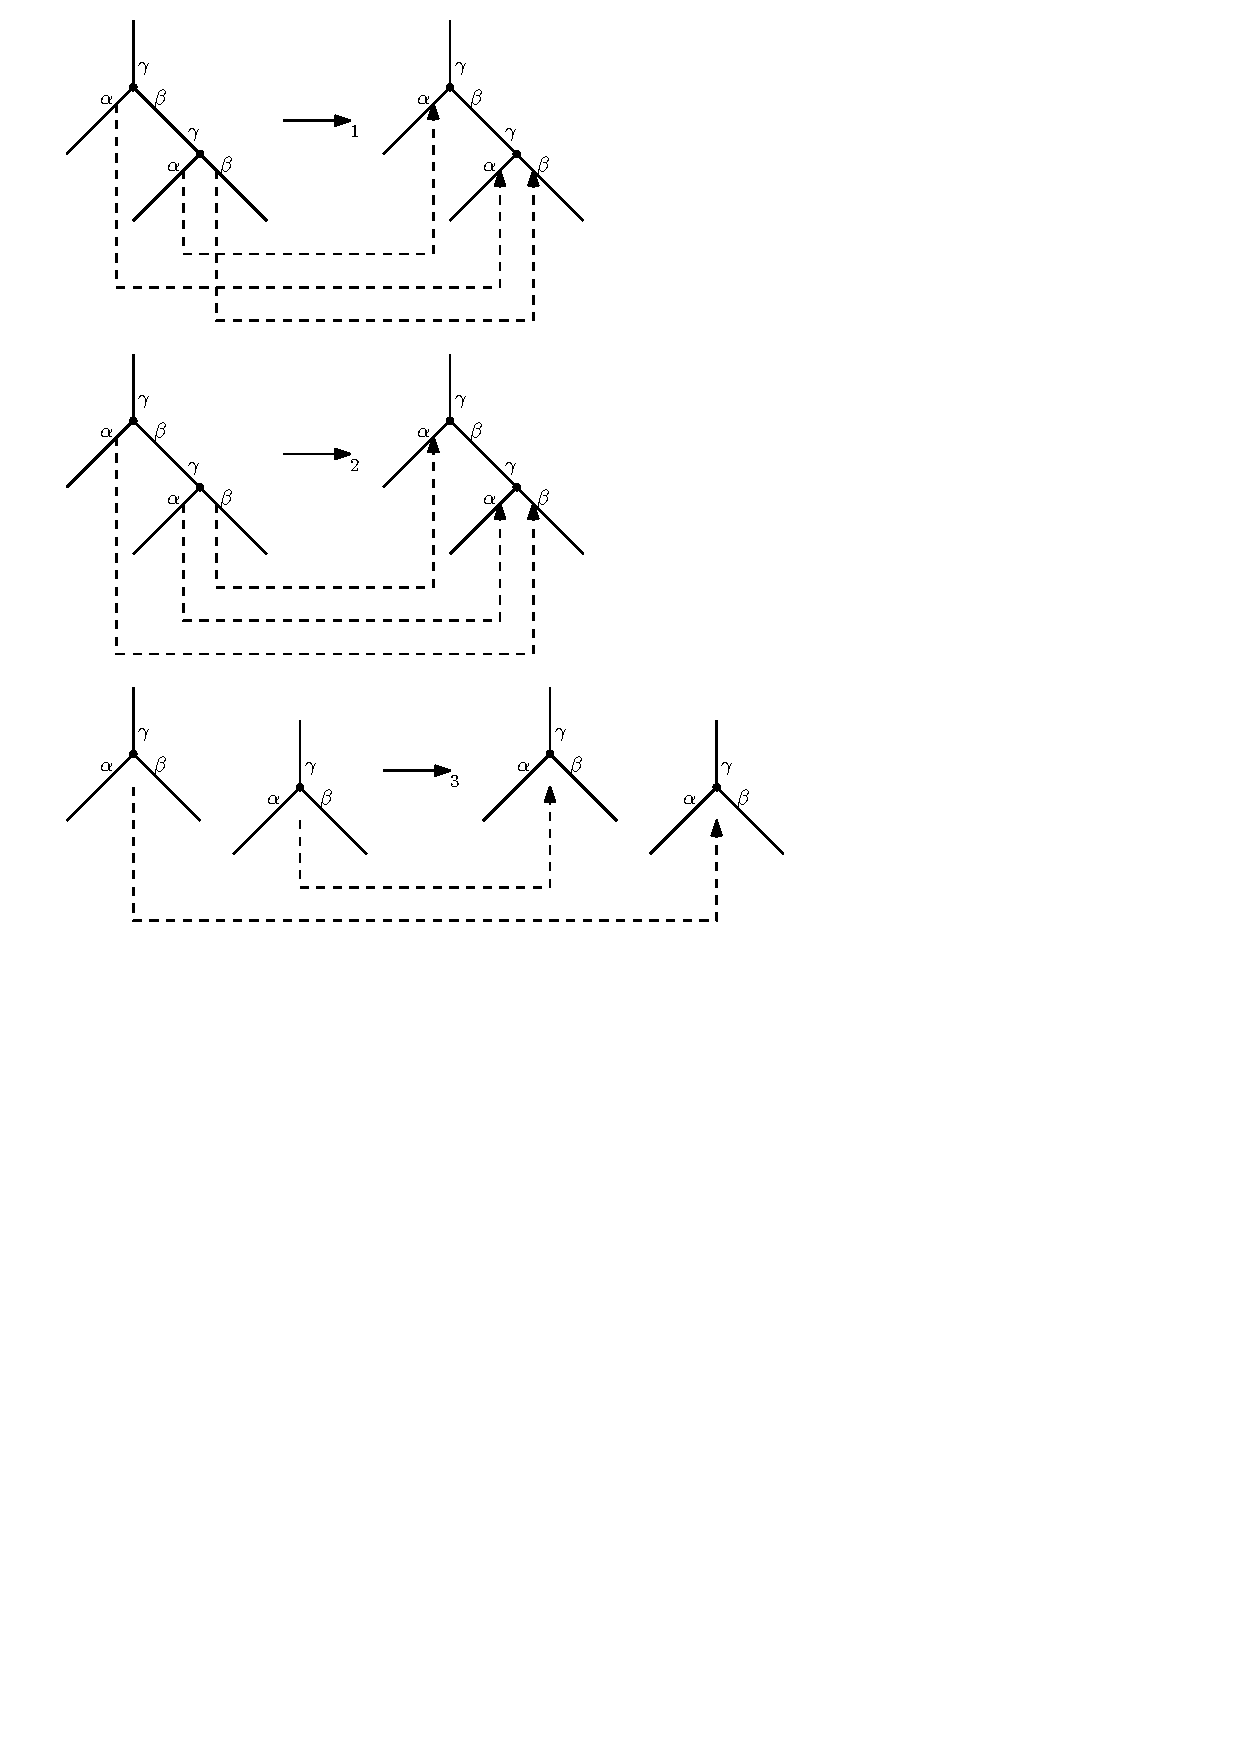
\includegraphics[width=0.7\textwidth]{grammar_rNNIu.pdf}
\caption{Graph grammar $\Gamma$ for $\rnniu$.
Maps $\to_i$ are shown by dashed lines.
In the first two productions, the edge-ends marked by $\beta$ and $\gamma$ without dashed lines are mapped to each other: top $\gamma$ to top $\gamma$, $\beta$ to $\beta$, bottom $\gamma$ to bottom $\gamma$.
In the last production, edge-ends marked by the same label are mapped to each other.
All pairs of nodes on both sides of each production must be of consecutive ranks.
The first two productions correspond to an $\nni$ move, while the last production corresponds to rank change.}
\label{grammar_rNNIu.pdf}
\end{figure}

The number of vertices in left sides of $\Gamma$ is $6$, the maximum number of vertices in any right side of a production of $\Gamma$ is $2$.
Since the number of internal nodes of a tree on $n$ leaves in $\rnniu$ is $n-1$, directly applying Theorem~2.3 from \autocite{Sleator1992-bp} we get the bound of $7^{n+2r-1}$.

This bound can be improved following the techniques described in Sections 3.2--3.4 of \autocite[][see also Section 5]{Sleator1992-bp} by bounding the number of possible productions available at a given time by a number smaller than their total.
Every node of a tree in any application of a production of grammar $\Gamma$ can play either of two roles: top node or bottom node.
Hence to indicate that a pair of nodes is ready for being destroyed and replaced using a production, we must specify which node is a top node and which is a bottom node.
We use a total of three node-labels (\textcite{Sleator1992-bp} call these ``labels of vertices'') to identify these two roles and to distinguish which of the two possible $\nni$ moves is applied.
We claim that three node-labels $a, b, c$ is enough to specify which productions can be applied to a given tree.
We must redefine the notion of readiness to verify this claim.
We say that a pair of consecutive nodes is \emph{ready} if the node-label of the bottom node is $a$ and the node-label of the top node is either $b$ or $c$.
If two consecutive nodes are ready and not connected by an edge in the tree, then only the rank move is possible.
If they are, the type of the move is determined by the node-label of the top node.
Hence, this notion of readiness uniquely identifies which of the three productions is applied.

\textcite{Sleator1992-bp} use a special node-label, called the ``zero label'', to mark nodes that should not be destroyed.
They also explain how to eliminate the zero label in various cases.
In our case, we can use one of the labels that are already in use, namely node-label $a$.
That is, to indicate that a node $v$ should never be destroyed, we label the node with an $a$.
This labeling will indeed preserve the node $v$ because of the following.
If $w$ is the node directly succeeding $v$ at some step of the derivation then $w$ can only be marked with an $a$ and hence the pair $v, w$ is not ready.
If $w$ is the node directly preceding $v$ at some step of the derivation then the pair $w, v$ is never ready.
Hence $v$ is preserved in either case.

Thus, all possible configurations encoded by the six nodes on the left sides of the productions of $\Gamma$ can be encoded using three node-labels.
This implies that the derivation can be encoded by a ternary sequence of length $n-1+2r$.
Indeed, the first $n-1$ entries of the sequence are needed to encode all possible node-labelings of the initial tree, plus two entries are needed for each of the $r$ applications of productions because every production creates two new nodes, each of which has to be node-labeled.
The number of such strings, $3^{n-1+2r}$, gives the desired improved bound.

The proof for the other three spaces follows similarly.
\DIFdelbegin \DIFdel{See Section~6.
\ Appendix for details}\DIFdelend \DIFaddbegin 

\DIFadd{For $\rnni$, we extend the graph grammar $\Gamma$ by two productions, namely, one for the move when two taxa swap their ranks and one for the move when a taxon and an internal node swap their ranks.
Since in both of these productions the only possible type of move is the rank move, two node-labels is enough for these productions.
Since the number of (internal and leaf) nodes in an $\rnni$ tree is $2n - 1$ and the maximum number of nodes on right sides of the productions is still $2$, the desired bound is $3^{2n-1 + 2r}$.
}

\DIFadd{For $\dttu$, we have to extend the grammar $\Gamma$ by two productions, namely, one for increasing the length of the branch between two nodes in the production and one for decreasing.
This increases the number of necessary node-labels by one.
Indeed, if a production has a long event interval on the left side, three node-labels are enough to indicate whether the event interval length increases or decreases.
Alternatively, if a production has a short event interval on the left side, three node-labels are needed for the top node to indicate the type of move to apply: a length increase move, one of the two possible $\nni$ moves, or a rank swap move.
Together, this requires $4$ node-labels and the desired bound is $4^{n-1 + 2r}$.
}

\DIFadd{For $\dtt$, we extend the grammar constructed for $\dttu$ by four productions, namely, one for the move when two taxa either swap their ranks or increase the interval length between them, one for the move when two taxa either increase or decrease the interval length between them, one for the move when a taxon and an internal node either swap their ranks or increase the interval length between them, and one for the move when a taxon and an internal node either increase or decrease the interval length between them.
All these moves require three node-labels, hence the desired bound is $4^{2n-1 + 2r}$}\DIFaddend .
\endproof

Since this theorem bounds the sizes of $r$-neighborhoods by functions of the form $a^{f(n) + 2r}$, the following corollary bounds the diameters of the graphs under consideration from below.

\begin{corollary}
Let $\Delta(\G)$, $|\G|$, and $\delta_r(\G)$ be the diameter, the number of vertices, and the number of vertices within distance $r$ from any given vertex in graph $\G$, respectively.
If $\delta_r(\G) = a^{f(n) + 2r}$ then
\[
\Delta(\G) \geq \frac 12 \log_a\frac{|\G|}{b},
\]
where $b = a^{f(n)}$.
In particular, $\Delta(\rnniu) \geq \frac 12 \log_3\frac{(n-1)!\,n!}{6^{n-1}}$.
\end{corollary}

\proof
We note that every $r$ that satisfies the inequality $\delta_r(\G) < |\G|$ is smaller than the diameter, that is, $\Delta(\G) > r$ for all such $r$.
By taking $\log_a(\cdot)$, the former inequality is equivalent to $\log_ab + 2r < \log_a|\G|$, that is, to $r < \frac 12 \log_a\frac{|\G|}{b}$.
Hence, the desired inequality.
\endproof


\subsection{Diameter of the graphs}

Now we estimate the diameter of the graphs from above, complementing the above lower bounds.
Recall that $\Delta(\G)$ is the diameter of graph $\G$.

\begin{theorem}
\label{diameterUpperBound}
For $n \ge 4$, $\Delta(\rnniu) \le n^2 - 3n - \displaystyle\frac 58$.
\end{theorem}

\proof
Let $T$ and $R$ be trees in $\rnniu$.
We show that there exists a path between them of length $n^2 - 3n - \frac 58$ or shorter.
We denote the taxa on one side from the root of $T$ by $A$ and the rest of the taxa by $B$.
Let $A = A_1 \cup A_2$ and $B = B_1 \cup B_2$ so that the root of $R$ splits the taxa into $A_1 \cup B_1$ and $A_2 \cup B_2$.
Note that all $A_i$'s and $B_i$'s have to be disjoint.
We assume that $|A_1| = |A_2| = |B_1| = |B_2| = \frac{n-1}{4}$ and denote this number by $s$.
We will see later in the proof that this assumption does not restrict the generality of our argument.

We construct the path from $T$ to $R$ proceeding in the following steps, which are illustrated on Figure~\ref{diameterUpperBound.pdf}.
Let $f(n)$ be the desired upper bound.
For move counts in the remainder of this proof, we will allow the ``null move'' in which no modification is made.

\begin{figure}
\centering
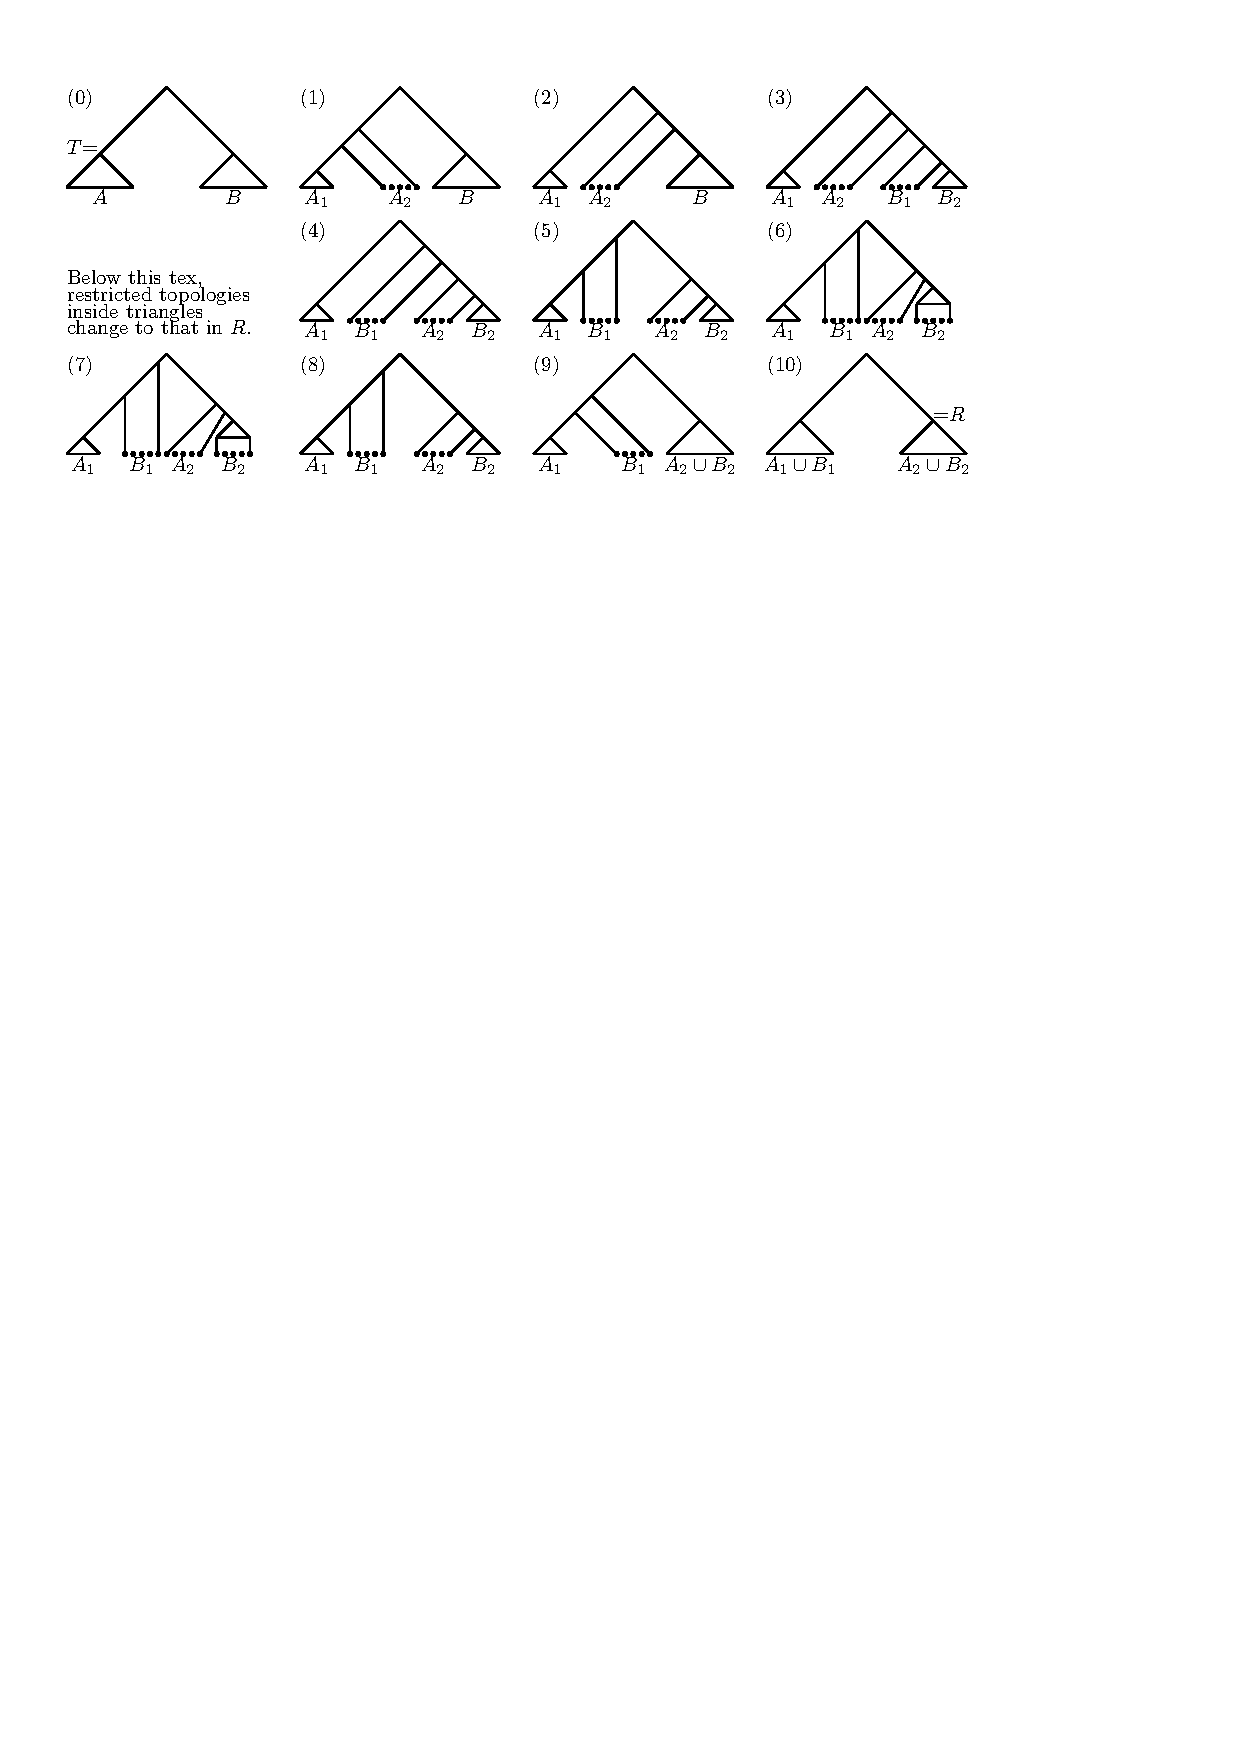
\includegraphics[width = \textwidth]{diameterUpperBound.pdf}
\caption{An algorithm to compute a (not necessarily shortest) path between discrete time-trees.
Although the trees at steps $(6)$ and $(7)$ look identical, the topologies inside the triangles are different: those at step $(6)$ correspond to the restriction of $T$, at step $(7)$---of $R$.}
\label{diameterUpperBound.pdf}
\end{figure}

 \begin{enumerate} [(1)]
\item Move all the nodes adjacent to taxa in $A_2$ on top of all the other nodes in $T$, apart from the root.
The tree restricted to $A_2$ is then a caterpillar tree.
This takes $3s^2$ moves.

\item Move the caterpillar tree on $A_2$ to the other side of the root.
This takes $\frac12 s^2 + \frac12 s$ moves.

\item Move all the nodes adjacent to taxa in $B_1$ on top of all nodes apart from those adjacent to taxa in $A_2$ and the root.
The tree restricted to $B_1$ is then a caterpillar tree.
This takes $2s^2$ moves.

\item Swap the caterpillars on $A_2$ and $B_1$.
This takes $s^2$ moves.

\item Move the caterpillar tree on $B_1$ to the other side of the root.
This takes $\frac12 s^2 + \frac12 s$ moves.

\item Translate the tree restricted to $B_2$ up to place it between the trees on $A_1$ and $A_2$.
This takes $s^2$ moves.

\item Convert the tree on $A_1 \cup B_2$ to the corresponding subtree in $R$ in terms of topology and relative ranking of nodes within the subtree.
This takes $2f(n/4)$ moves.

\item Translate the tree on $B_2$ down so that the tree on $A_1 \cup B_2$ matches the corresponding subtree in $R$ in terms of topology and relative ranking of nodes.
This takes $s^2$ moves.

\item Merge the tree on $A_2$ with the tree on $B_2$ so that the tree on $A_1 \cup A_2 \cup B_2$ coincides with that in $R$.
This takes $2s^2$ moves.

\item Merge the tree on $B_1$ with the tree on $A_1$ so that the tree coincides with $R$.
This takes $3s^2$ moves.
 \end{enumerate} 

In total, we have a recursive equation $f(n) = 14s^2 + s + 2 f(n/4)$.\\
Assuming that the solution is a polynomial, we see that the polynomial must be of degree $2$.
It remains to apply the recursive equation to find the coefficients of the polynomial:
\[
f(n) = n^2 - 3n - \frac 58.
\]

It remains to note that the assumption $|A_1| = |A_2| = |B_1| = |B_2| = \frac{n-1}{4}$ does not increase the distance between $T$ and $R$.
Indeed, the sets can be chosen so that at most half of the nodes have to cross the root, that is, $|A_2 \cup B_1| \le \frac{n-1}{2}$.
Furthermore, the smaller the size of $A_2 \cup B_1$ the shorter the path.
Finally, the total length of the path is maximized when $|A_2| = |B_1|$ and $|A_1| = |B_2|$.
\endproof

Although we stated and proved the theorem only for the $\rnniu$ graph, the idea can be adapted to the other graphs considered here.
However, this adaptation goes beyond the scope of this paper.
%DIF < TODO: Add this for the full version?

We also note that the proof of the theorem provides an efficient algorithm for computing (not necessarily shortest) paths between discrete time-trees.
This algorithm can be used for efficient exploration of the space, e.g.\ via MCMC, where approximate paths can be used to improve mixing by making distant proposals.
The algorithm might also be useful to determine if two trees appear to be separated by a valley (e.g.\ of posterior probability) or if they are rather located on a plateau.

A non-ranked tree has a symmetry associated with every internal node.
Those symmetries can be employed to consider only a single representative from equivalent pairs of trees, such as by using tanglegrams \autocite{Matsen2015-fn, Whidden2015-es}\DIFaddbegin \DIFadd{, where a }\emph{\DIFadd{tanglegram}} \DIFadd{is a graph formed by identifying the leaves of two phylogenetic trees}\DIFaddend .
However, as the following proposition shows, ranked trees are free from all but one of those symmetries, hence the tanglegram approach is not applicable in this case.

\begin{proposition}
Let $T$ be a tree from $\dtt$, $\dttu$, $\rnni$, or $\rnniu$ and $\sigma$ a permutation of taxa of $T$.
Let $T_\sigma$ be the tree obtained from $T$ by permuting the taxa using $\sigma$.
Then $T = T_\sigma$ if and only if $\sigma$ is either the identity permutation or a transposition of a pair of taxa that form a cherry \DIFdelbegin \footnote{\DIFdel{A }\emph{\DIFdel{cherry}} %DIFAUXCMD
\DIFdel{is a pair of taxa adjacent to a common internal node in the tree.}}
%DIFAUXCMD
\addtocounter{footnote}{-1}%DIFAUXCMD
\DIFdelend in $T$.
\end{proposition}

\proof
The sufficiency is obvious.
For the necessity, assume that $\sigma$ transpose taxa $i,j$ such that $i,j$ is not a cherry in $T$.
This implies that $i$ and $j$ have different parents.
Hence $T \ne T_\sigma$ because the ranks of the parent of $i$ are different in $T$ and $T_\sigma$.
\endproof

These observations suggest that the $\nni$ graph is geometrically and algorithmically different from the other four graphs.

\iftoggle{curvatureON}{
\section{Ricci-Ollivier curvature of discrete time-trees}

We need the following corollaries for our analysis of curvature.

\begin{corollary}
\label{degreeBounds}
The following are satisfied in $\dtt$ for every pair of trees $T$ and $R$.
\begin{align*}
& \deg(T)-\deg(R) \leq 3n-4					&& \mbox{in $\dtt$,}\\
& \deg(T)-\deg(R) \leq 2n-4					&& \mbox{in $\dttu$,}\\
& \deg(T)-\deg(R) \leq 2n-3					&& \mbox{in $\rnni$,}\\
& \deg(T)-\deg(R) \leq n-3					&& \mbox{in $\rnniu$,}\\
& \dfrac25 < \dfrac{\deg(T)}{\deg(R)} < \dfrac52		&& \mbox{in $\dtt$,}\\
& \dfrac13 < \dfrac{\deg(T)}{\deg(R)} < 3			&& \mbox{in $\dttu$ and $\rnni$,}\\
& \dfrac12 < \dfrac{\deg(T)}{\deg(R)} < 2			&& \mbox{in $\rnniu$,}\\
\end{align*}
and all inequalities are tight.
\end{corollary}

\proof
The first four inequalities follow from Lemma~\ref{neighBound} immediately.

For the fifth inequality we note that
\[
\frac{\deg(T)}{deg(R)} \geq \frac{2(n-1)}{5n-6} = \frac25 \left(1 + \frac{1}{5n-6}\right) \searrow \frac 25 \mbox{ when } n\to\infty
\]
The upper bound follows similarly, as well as the rest of inequalities.
\endproof

For $\nni$ graph, Lemma~\ref{neighBound} implies that $deg(T)-deg(R) = 0$ and $\frac{\deg(T)}{deg(R)} = 1$.

Let $N(T)$ be the set of trees at distance one from $T$, that is, the set of trees adjacent to $T$ in the corresponding graph.
The following lemma describes how many trees the tree neighborhoods can have in common.

\begin{lemma}
\label{intersecNeighb}
The following is true for all the graphs $\nni$, $\rnni$, $\rnniu$, $\dtt$, and $\dttu$.
If $d(T,R) = 1$ then $|N(T)\cap N(R)|\in\{0,1\}$.
\end{lemma}

\proof
Suppose $T$ and $R$ are neighbors.
If the trees differ by a single branch length or rank change then the fact that $\nni$ moves only apply to short branches implies that any shared neighbor $S$ would have to match the length or rank of one of the trees.
As $S$ must differ from both trees, they do not have a neighbor in common.
If $T$ and $R$ are $\nni$-neighbors, there is precisely one tree which is a neighbor of both $T$ and $R$, namely the third tree that can be obtained by resolving the interval that connects $T$ and $R$.
\endproof

The following general lemma is true for all graphs, particularly, for those we consider in this paper.
By \emph{distance-one random walk}, we mean a random walk $(m_x)_{x \in X}$ satisfying $m_x(y) = 0$ for all $x$ and $y$ such that $d(x,y) > 1$.

\begin{lemma}
\label{curvBoundGeneral}
Let $(M,d)$ be a finite metric space and $x,y$ a pair of points from $M$.
If $(m_x)_{x \in M}$ is a distance-one random walk on $M$, then the curvature $\kappa$ of the random walk satisfies the following boundary conditions.
\[
\dfrac{-2}{d(x,y)} \leq \kappa(x,y) \leq \dfrac{2}{d(x,y)}.
\]
\end{lemma}

\proof
Let $x$, $y$, $u$, and $v$ be arbitrary points from $M$ such that both $m_x(u)$ and $m_y(v)$ are positive.
Since $m$ is a distance-one random walk, $d(u,v) \leq d(x,y) + 2$.
Hence for any coupling $\{p_{u,v}\}$,
\[
W(m_x,m_y) \leq \sum p_{u,v} d(u,v) \leq (d(x,y)+2)\sum p_{u,v} = d(x,y) + 2,
\]
where the sum is taken over a correspondence between the set of $u \in N(x)$ and $v \in N(y)$.
So, $\kappa(x,y) \geq - 2/d(x,y)$.
The lower bound follows similarly from $d(u,v) \geq d(x,y) - 2$.
\endproof

Note that this lemma can be generalized to \emph{distance-$d$} random walks, which are those satisfying $m_x(y) = 0$ for all $x$ and $y$ such that $d(x,y) > d$.
In this case, using the notations of the lemma, $d(u,v) \leq d(x,y) + 2d$.
Thus,
\[
-\dfrac{2d}{d(x,y)} \leq \kappa(x,y) \leq \dfrac{2d}{d(x,y)}.
\]

As we will see in the next few lemmas, these bounds can be improved for certain random walks on the graphs under consideration.

\begin{lemma}
\label{uniformUpper}
Let $T$ and $R$ be adjacent trees.
Then the curvature of the following spaces with uniform random walk satisfy
\begin{align*}
& \kappa(T,R) \leq \dfrac{1}{2(n-1)}	&& \mbox{for $\dtt$,}\\
& \kappa(T,R) \leq \dfrac{1}{2(n-2)}	&& \mbox{for $\nni$, and}\\
& \kappa(T,R) \leq \dfrac{1}{n-1}	&& \mbox{for $\rnni$, $\rnniu$, and $\dttu$.}
\end{align*}
The bounds are tight.
\end{lemma}

\proof
To maximize the curvature $\kappa(T,R)$, we have to minimize $W(m_T,m_R) = \inf\limits_{\mu\in\M} \sum\limits_{x,y\in V}\mu(x,y) d(x,y)$.
The latter is minimized when the probability mass $\mu(x,y)$ to be moved at shorter distance $d(x,y)$ is maximized.
Since $d(T,R) = 1$, it follows from Lemma~\ref{intersecNeighb} that the smallest possible value of $d(x,y)$ is $0$ (the case when $|N(T) \cap N(R)| = 1$).
Hence, to maximize the curvature we are to maximize the probability mass allocated to the tree $E$ in the intersection $N(T) \cap N(R)$.
It follows from Lemma~\ref{neighBound} that the maximal mass $p_E$ we can allocate under a uniform random walk to the tree $E$ is $\frac{1}{2(n-1)}$ in $\dtt$, $\frac{1}{2(n-2)}$ in $\nni$, and $\frac{1}{n-1}$ in $\rnni$, $\rnniu$, and $\dttu$.
It is not hard to see that trees $T$ and $R$ can be chosen so that $d(x,y) = 1$ for all $x,y$ which are different from $E$ and for which $\mu(x,y) > 0$.
Hence, $\kappa(T, R) = 1 - \left(\sum\limits_{x,y\in V\setminus\{E\}}\mu(x,y)\cdot 1 + p_E \cdot 0\right) = 1 - (1-p_E) = p_E$.
The lemma follows.
\endproof

This lemma and corollary provide tighter upper bounds for the curvature than Lemma~\ref{curvBoundGeneral} for all $n$.

It is easy to generalize the lemma to the uniform $p$-lazy random walk.
Indeed, we observe that the curvature between adjacent trees $T$ and $R$ under a uniform $p$-lazy random walk satisfies
\begin{align*}
& \kappa(T,R) \leq \frac{p}{2(n-1)}	&& \mbox{in $\dtt$,}\\
& \kappa(T,R) \leq \frac{p}{2(n-2)}	&& \mbox{in $\nni$, and}\\
& \kappa(T,R) \leq \frac{p}{n-1}	&& \mbox{in $\rnni$, $\rnniu$, and $\dttu$.}
\end{align*}

We recall that the \emph{asymptotic Ricci-Ollivier curvature} \autocite{Loisel2014-gu} $\ric$ of a metric space with uniform $p$-lazy random walk is defined by
\[
\ric(x,y) = \lim_{p\to0} \frac{\kappa(x,y)}{p}
\]

In this case the asymptotic curvature between adjacent trees in $\dtt$ with uniform $p$-lazy random walk is bounded from above by
\[
\frac{1}{2(n-1)}
\]

Following \textcite{Loisel2014-gu}, we will refer to non-asymptotic curvature as \emph{coarse curvature} to distinguish between the two alternative notions of curvature.

Thus, the upper bounds of asymptotic curvatures of $\nni$, $\rnni$, $\rnniu$, $\dtt$, and $\dttu$ spaces coincides with the coarse curvatures of the spaces.

We continue with lower bounds on curvature of spaces with uniform lazy random walks.

\begin{lemma}
\label{uniformLower}
Let $T$ and $R$ be adjacent trees.
Then both the asymptotic curvature of the space with $p$-lazy uniform random walk and the curvature of the space with uniform random walk are at least
 \begin{enumerate} [(i)]
\item $-\dfrac{4}{n-1}$ in $\dtt$,
\item $-\dfrac{4}{n-2}$ in $\nni$,
\item $-\dfrac{8}{n-1}$ in $\rnni$.
 \end{enumerate} 

The bounds are tight.
\end{lemma}

\proof
Let $T$ and $R$ be two adjacent trees.
To minimize the curvature, we have to maximize $W(m_T, m_R)$ across $T$ and $R$.
The latter is maximized when the probability mass on trees $E\in N(T)$ such that $d(E, N(R)) > d(T, R)$, is
maximized\footnote{If $x$ is a point of a metric space $(M,d)$ and $S \subseteq M$ then by $d(x,S)$ we denote $\inf\limits_{s \in S} d(x,s)$.}.
Since $d(T, R) = 1$, the maximum possible number of such trees $E$ is
\todo{Explain this.
EM skipped pending explanation.}
$8$.
To make $W(m_T,m_R)$ being as large as possible, we have to assume $d(S, N(R)) = 1$ for the rest of the trees $S$ from $N(T)$.
Hence for the uniform random walk we have:
\[
W(m_T,m_R)\leq 8 \cdot 2 \cdot \frac{1}{|N(T)|} +
(|N(T)| - 8) \cdot \frac{1}{N(T)} = 1 + \dfrac{8}{|N(T)|}.
\]
Hence, $\kappa(T,R) = 1 - W(m_T,m_R) \geq - \dfrac{8}{|N(T)|}$.

A similar reasoning applies for the $p$-lazy random walk:
\[
W(m_T,m_R)\leq 8 \cdot 2 \cdot \frac{p}{|N(T)|} +
(|N(T)| - 7) \cdot \frac{p}{|N(T)|} + (1-p) - \frac{p}{|N(T)|} =
\]
$1 + \dfrac{8p}{|N(T)|}$.
Hence, $\ric(T,R) = \lim\limits_{p\to0}\left(1 - W(m_T,m_R)\right) \geq - \dfrac{8}{|N(T)|}$.

It remains to note that Lemma~\ref{neighBound} gives us an estimate $|N(T)| \geq 2(n-1)$ in $\dtt$, $|N(T)| \geq 2(n-2)$ in $\nni$, and $|N(T)| \geq n-1$ in $\rnni$.
The lemma follows.
\endproof

\begin{corollary}
\label{flatInLimDTS}
Let $(T_n,R_n)_{n\in\omega}$ be a sequence of pairs of trees such that $d(T_n,R_n) = 1$ in $\nni$, $\rnni$, or $\dtt$.
Then $\lim\limits_{n \to \infty}\kappa(T_n,R_n) = \lim\limits_{n \to \infty}\ric(T_n,R_n) = 0$.
\end{corollary}

\proof
Follows from Lemma~\ref{uniformUpper} and Lemma~\ref{uniformLower}.
\endproof

As we have just proved, the corollary above holds true in $\nni$, $\rnni$, and $\dtt$.
This corollary is also true in the SPR graph of rooted trees \autocite{Whidden2015-es}.
Actually, this property can be derived from the following general statement for all spaces mentioned, as well as for many others.

\begin{proposition}
\label{flatInLimGen}
Let $(M_n,d_n)_{n \in \omega}$ be a sequence of finite metric spaces and $(x_n, y_n)$ a sequence of adjacent vertices from $M_n$, that is $d_n(x_n,y_n) = 1$, such that
 \begin{enumerate} [(1)]
\item
\label{intersec}
$\big|N(x_n) \cap N(y_n)\big| = o(|N(x_n)|)$
\item
\label{difference}
$\big||N(x_n)| - |N(y_n)|\big| = o(|N(x_n)|)$
\item
\label{dist2}
$\big|\{(x,y) \mid
	x \in N(x_n),~ y \in N(y_n),~ d(x, y) \geq 2\}\big| = o(|N(x_n)|)$
 \end{enumerate} 

Then $\lim\limits_{n \to \infty} \kappa(x_n, y_n) = 0$.
\end{proposition}

\proof
Consider an arbitrary $n$ and the pair of points $x_n,y_n$.
Set $I_0 = N(x_n) \cap N(y_n)$, denote by $I_1$ the set of points $z$ such that the probability mass is moved from $z$ at distance one under the optimum coupling for $W(m_{x_n},m_{y_n})$, by $I_2$ the set of points $z$ such that the probability mass is moved from $z$ a distance $\geq 2$ under the optimum scenario for $W(m_x,m_y)$.
Then
\[
W(m_{x_n},m_{y_n}) = \sum_{I_0} d_i x_i p_{x_i} + \sum_{I_1} d_i x_i p_{x_i} +
\sum_{I_2} d_i x_i p_{x_i}.
\]
It follows from~(\ref{intersec}) and~(\ref{dist2}) that the first and the last sums are $\O(1)$ when $n\to\infty$.
This together with property~(\ref{difference}) implies that the middle sum tends to $1$ when $n\to\infty$ because the number of points $z$ such that the probability mass has to travel at distance one under an optimum scenario, divided by $|N(x_n)|$, tends to $1$ when $n\to\infty$.
\endproof

We note that in both Corollary~\ref{flatInLimDTS} and Proposition~\ref{flatInLimGen}, the assumption of being at distance one can be relaxed by that of being at a distance uniformly bounded by a slowly growing function.
But since the primary focus of this paper is on the spaces under consideration, we will not \todo{Should we?} include the statement in general terms of metric spaces.
However, we prove below (Theorem~\ref{zero-in-the-limit}) a much stronger property of the spaces, namely, that the curvature tends to zero when the tree size tends to infinity does not matter what distance between the trees is.
}
{}

\iftoggle{curvatureON}{
We now use Theorem~\ref{max_good_neighbors} to prove the following.

\todo[inline]{$\downarrow$ This must be true for $p$-lazy walk as well.}

\begin{theorem}
\label{zero-in-the-limit}
Let $(T_n,R_n)_{n\in\omega}$ be a sequence of pairs of $\dtt_2$-trees on $n$ taxa.
Then $\lim\limits_{n \to \infty}\kappa(T_n,R_n) = 0$ for the uniform random walk.
\end{theorem}

\proof
Since the curvature is a local property, it follows from Lemma~\ref{uniformLower} that $\kappa(T_n,R_n) \geq -\dfrac{4}{n-1}$ for all $n$.
To finish the proof, we need to bound the sequence $\kappa(T_n,R_n)$ from above by another sequence which tends to zero.

Let us fix an $n$ and let $U$ be the set of trees $E \in N(T)$ such that $d_\dtt_2(E,R_n) \leq d_\dtt_2(T_n,R_n)$ as in Theorem~\ref{max_good_neighbors}, and $B$ be the rest of trees $N(T_n)\setminus U$ from $N(T_n)$.
Let's denote $d_\dtt_2(T_n,R_n)$ by $d$.
Then
\[
W(m_{T_n},m_{R_n}) = \sum_{i\in U} p_i d_i + \sum_{j\in B} p_j d_j \geq
\sum_{i\in U} p_i (d-2) + \sum_{j\in B} p_j d =
\frac{|U|(d-2)}{|N(T_n)|} + \frac{|B|d}{|N(T_n)|}.
\]
Hence,
\[
\kappa(T_n,R_n) = 1 - \frac{W(m_{T_n},m_{R_n})}{d} \leq
1 - \frac{|U| + |B|}{|N(T_n)|} + \frac{2|U|}{|N(T_n)|d}
= \frac{2|U|}{|N(T_n)|d}.
\]
It follows from Theorem~\ref{max_good_neighbors} that $|U| \leq 4d$.
Thus, $\kappa(T_n,R_n) \leq \dfrac{8}{|N(T_n)|}$.
It remains to note that $\lim\limits_{n\to\infty}\dfrac{8}{|N(T_n)|} = 0$.
\endproof

Clearly, the same reasoning goes through for the other three spaces under consideration:

\begin{corollary}
Let $(T_n,R_n)_{n\in\omega}$ be a sequence of pairs of trees on $n$ taxa.
Then $\lim\limits_{n \to \infty}\kappa(T_n,R_n) = 0$ for $\nni$, $\rnni$, and $\dtt$ distances.
\end{corollary}

We now estimate the curvature of the Metropolis-Hastings random walk, which proposes a tree in the $1$-neighborhood uniformly at random and accepts the proposal with probability $\min\left(1, \dfrac{|N(T_{old})|}{|N(T_{new})|}\right)$.
We denote the corresponding curvature by $\kappa(\MH;T,R)$.

\begin{lemma}
The following inequalities are satisfied in both $\dtt_2$ and $\dtt$.
\[
\kappa(T,R) - \dfrac{6}{5d(T,R)} \leq \kappa(\MH;T,R) \leq \kappa(T,R) +
\dfrac{6}{5d(T,R)}\mbox{, and}
\]
\[
\kappa(T,R) - \dfrac35 \leq \kappa(\MH;T,R) \leq \kappa(T,R) + \dfrac35.
\]
\end{lemma}

\proof
From Corollary~\ref{degreeBounds} we have that $\frac{|N(T_{old})|}{|N(T_{new})|} \geq \frac{2}{5}$, so the probability mass that an MH move leaves at $T_{old}$ is not greater than $\frac35$.
The rest of the proof follows \autocite[][Proof of Lemma~V.8]{Whidden2015-es} literally.
\endproof

\begin{corollary}
The following inequalities are satisfied in $\rnni$ \todo{What about NNI?}.
\[
\kappa(T,R) - \dfrac{4}{3d(T,R)} \leq \kappa(\MH;T,R) \leq \kappa(T,R) +
\dfrac{4}{3d(T,R)}\mbox{, and}
\]
\[
\kappa(T,R) - \dfrac23 \leq \kappa(\MH;T,R) \leq \kappa(T,R) + \dfrac23.
\]
\end{corollary}

\proof
Use Corollary~\ref{degreeBounds}.
\endproof
}{}


\subsection{Efficient algorithm for generating $\rnni$ graphs}

We now introduce an algorithm to compute the $\rnni$ graph on $n$ leaves by extending an algorithm from \DIFdelbegin \DIFdel{\textcite{Whidden2015-es}}\DIFdelend \DIFaddbegin \autocite{Whidden2015-es}\DIFaddend .
The input to our algorithm is a set $S$ of $\rnni$ trees in the format described by \textcite{Gavryushkin2014-bw} and implemented in \autocite{tauGeodesic} (see also \autocite{Semple2003-nj}).
The two key requirements of the algorithm are the ability to enumerate the neighbors of a given tree in the $\rnni$ graph, and the ability to determine whether a given tree is already a vertex of the graph.
Both of these requirements follow from an efficient unique representation for ranked trees.

A node of a tree is given by the set of taxa that are all descendants of the node.
A tree is then given by a sequence of nodes ordered by their ranks.
Clearly, this obtained representation is unique.
For example, the representation of the tree on Figure~\ref{timeTree.eps} is $(\{A\}, \{C\}, \{D\}, \{B\}, \{E\}, \{A,B\}, \{D,E\}, \{C, D, E\}, \{F\}, \{A,B,F\}, \{A,B,C,D,E,F\})$, or
$(\{A,B\}, \{D,E\}, \{C, D, E\}, \{A,B,F\}, \{A,B,C,D,E,F\})$ if we make the tree ultrametric by placing all taxa below the most recent divergence event.
Using this representation of trees we construct a map $\nu : S \to \omega$, where $\omega$ is the set of non-negative integers.
This map allows us to determine whether or not a tree is already a vertex of the graph.
This takes linear time if the map is implemented as a trie.
We can also enumerate the neighbors of a tree in $O(n^2)$-time using Lemma~\ref{neighBound}.
The algorithm therefore takes $O(|S|*n^2)$-time.
The high-level steps of the algorithm are as follows.
See \DIFdelbegin \DIFdel{\mbox{%DIFAUXCMD
\cite{Whidden2015-es} }%DIFAUXCMD
}\DIFdelend \DIFaddbegin \autocite{Whidden2015-es} \DIFaddend for an analogous proof of correctness.

\medskip

\textsc{Construct-$\rnni$-Graph($S$)}
 \begin{enumerate} [1.]
	\item Let $G$ be an empty graph.
	\item Let $\nu$ be an empty mapping from trees to integers.
	\item Let $i = 0$.
	\item For each of the $m$ trees: \vspace{-0.2em}
		 \begin{enumerate} 
			\item Add a vertex $i$ to $G$ representing the current tree $T_i$.
			\item Add $T_i \rightarrow i$ to $\nu$.
			\item For each neighbor $T_j$ of $T_i$:
				 \begin{enumerate} 
					\item[(j)] If $T_j$ is in $\dom(\nu)$ then add an edge $(i, \nu(T_j))$ to $G$.
				 \end{enumerate} 
		\item $i = i + 1$.
		 \end{enumerate} 
 \end{enumerate} 

\iftoggle{curvatureON}{
\section{Some other spaces}

Several important proposal mechanisms used in phylogenetic Bayesian inference by popular software packages such as BEAST2 \autocite{beast2} favor topological moves or tree moves depending on various conditions.
All tree moves we have been considering so far do not make an explicit distinction between topological changes and branch length changes.
To address this issue\todo{issue?}, we consider the following tree move that explicitly allows distributing the acceptance probability between topological and branch length moves.

{\bf Lazy walk.}
Let $p$ be the laziness probability, that is, we do nothing with probability $1-p$ and distribute the probability $p$ as follows.
We decide first on what type of move we want to perform: choose a topological move with probability $q$ and a length move otherwise, that is, $q \leq p$ and the probability of a length move is $p-q$.
The proposal is rejected if a topological move is impossible.

{\bf tau move.}
Choose a coordinate uniformly at random.
Increase the coordinate by $1$ with probability $p$ and decrease it by $1$ otherwise.
If the coordinate becomes $0$, resolve the multifurcation uniformly at random and set the new coordinate to $1$.
Note that this mechanism does not bound edge lengths from above and favors topological moves when $p<1/2$.
}{}


\section{Open problems and conjectures}

In the previous section we posed Problem~\ref{problemComplexity}, which asks about the complexity of computing the distance in discrete time-tree graphs.
This problem is the primary obstacle for actual biological applications of the introduced graphs.
The history of research into computational complexity of phylogenetic graphs is very rich and exciting, in particular for the case of the $\nni$ graph, with a number of erroneous results being published over the 25 years it took to settle the complexity.
See \autocite{Dasgupta2000-xa} for a detailed discussion of those publications, some of which claimed that $\nni$ distance is NP-hard while others claiming that $\nni$ distance is decidable in polynomial time.
The latter claims were mainly based on the so-called Split Theorem which states the following:
If a partition of leaves given by an edge is shared between two trees then there exists a shortest $\nni$ path between the trees such that every tree on the path maintains the partition.
These claims were finally refuted by \textcite{li1996some}, who proved that the Split Theorem does not hold in the $\nni$ graph.
Hence, a natural question that would contribute to understanding Problem~\ref{problemComplexity} is whether or not the Split Theorem holds in the $\rnni$ graph and other time-tree graphs.


\subsection{Split Theorem}

\textcite{li1996some} used properties of the diameter of the $\nni$ graph and the sizes of its neighborhoods to provide an example of trees such that every shortest $\nni$ path between the trees fails to maintain a partition of taxa shared by the origin and destination trees.
Specifically, they showed that sorting two caterpillar trees simultaneously is more efficient than sorting them independently, provided the size of the trees is large enough.
In the following, we conjecture that the ranked versions of $\nni$ graph maintain splits along shortest paths.
Our conjecture is based on the fact that $\rnni$ does not satisfy the diameter bounds necessary for the argument in \autocite{li1996some} to go through---see Theorems~\ref{neighSizeTh} and~\ref{diameterUpperBound}.
Indeed, since sorting a caterpillar tree of size $k$ in $\rnni$ takes fewer moves than merging two such caterpillar trees and then separating them, the counter-example from \autocite{li1996some} does not apply in $\rnni$.
This counter-example using two trees encodes the basic way in which $\nni$ shortest paths are non-trivial: that one can economize by first grouping leaves into bundles, moving the bundles, and then breaking the bundles apart.
Because this basic operation does \DIFaddbegin \DIFadd{not }\DIFaddend provide an advantage in the simplest case of two caterpillar trees \DIFaddbegin \DIFadd{in $\rnni$}\DIFaddend , we do not believe that it will hold for more complex collections of moves.

\begin{conjecture}
\label{conjSplit}
The following is true in all graphs $\dtt$, $\dttu$, $\rnni$, and $\rnniu$, but not in $\nni$.
If a partition of leaves given by an edge is presented in two trees $T$ and $R$ then the partition is presented in every tree on every shortest path between $T$ and $R$.
\end{conjecture}


\subsection{Computing the distance}

In this section, we bound the number of neighbors of a tree $x$ in the discrete time-tree graphs that are closer than $x$ to a given tree $y$, \textbf{under the assumption that Conjecture~\ref{conjSplit} holds}.
\DIFdelbegin \footnote{\DIFdel{We denote trees by lowercase letters to stress the fact that we are considering graphs as metric spaces in this section.}}
%DIFAUXCMD
\addtocounter{footnote}{-1}%DIFAUXCMD
\DIFdelend \DIFaddbegin \DIFadd{We denote trees by lowercase letters to stress the fact that we are considering graphs as metric spaces in this section.
}\DIFaddend We show that the maximum fraction of neighbors that tend closer to $y$ grows linearly with respect to $d(x,y)$.
\iftoggle{curvatureON}{
These subsets of neighbors are the force pushing towards positive curvature, so this will allow us to bound the maximum curvature with respect to distance.
}{
When the graph is seen as a metric space, this property is important for the study of the curvature of the space as well as convergence properties of random walks over the space.
This will be useful in future studies analogous to \autocite{Whidden2015-es}.
Furthermore, the result provides a further insight into possible approaches to Problem~\ref{problemComplexity}.
}

\begin{theorem}
\label{max_good_neighbors}
Assume that Conjecture~\ref{conjSplit} holds.
Let $x$ and $y$ be two trees and $N(x)$---a one-neighborhood of $x$.
Then the number of trees $u \in N(x)$ such that $d(u, y) \le d(x, y)$ is at most
 \begin{enumerate} [(i)]
\item $3d(x,y)$ in $\rnni$,
\item $4d(x,y)$ in $\dtt_2$,
\item $5d(x,y)$ in $\dtt_m$ for $m > 2$.
 \end{enumerate} 
\end{theorem}

\DIFdelbegin \DIFdel{The proof of this theorem can be found in Section~6.
\ Appendix.
}\DIFdelend \DIFaddbegin \proof
\DIFadd{We first prove the statement for $\dtt_2$.
Let $U$ be the set of neighbors $u$ of $x$ such that $d(u,y) \le d(x,y)$, as stated in the theorem.
We partition $U$ into three sets of trees---$I$, $R$, and $L$---obtained from $x$ by a single $\nni$ move, rank change, or length change, respectively.
We then prove the theorem by bounding the size of each partition by $2d(x,y)$, $d(x,y)$, and $d(x,y)$, respectively.
}

\DIFadd{We first consider some basic properties of minimal length paths between $x$ and $y$.
Observe that at most $d(x,y)$ bipartitions differ between $x$ and $y$, as each $\nni$ operation replaces one bipartition with another (and rank and length changes do not modify bipartitions).
Now, Conjecture~\ref{conjSplit} implies that no minimal length path from $x$ to $y$ will replace a bipartition that is common to $x$ and $y$.
}

\DIFadd{We are now ready to bound the sizes of each partition $I$, $R$, and $L$.
First, consider the subset $I$ of closer neighbors obtained via $\nni$ moves.
By our observations above, $|I|$ is bounded by the number of $\nni$ operations that modify one of the at most $d(x,y)$ bipartitions of $x$ that are not a bipartition of $y$.
There are two neighbors of $x$ that lack any given bipartition (obtained by moving either the left or right subtree located below the bipartition).
Therefore, $|I| \le 2d(x,y)$.
}

\DIFadd{Second, consider the subset $R$ of closer neighbors obtained via rank change moves.
These operate either on one of $x$'s unique bipartitions or a bipartition common to $x$ and $y$ that differs in rank.
As observed above, the number of unique bipartitions is bounded by the maximum number of $\nni$ moves on any minimal $x$ to $y$ path.
Any such path must fix the ranks of each common edge.
In other words, if $r_1$ is the number of trees in $U$ which are obtained from $x$ by a rank move corresponding to a common edge and $r_2$ is the number of trees in $U$ which are obtained from $x$ by a rank move corresponding to a unique edge of $x$, then $r_1 + r_2 \leq d(x,y)$, because the $r_1$ moves have to be done along every shortest path from $x$ to $y$.
Thus, the total size of $R$ is bounded by $d(x,y)$.
}

\DIFadd{The bound of $d(x,y)$ on the number of length changes that can be applied to move $x$ closer to $y$ follows similarly.
Therefore, there are at most $|I| + |R| + |L| \le 2d(x,y) + d(x,y) + d(x,y) = 4d(x,y)$ trees $u \in N(x)$ such that $d(u, y) \le d(x, y)$.
}

\DIFadd{The statement for the other two graphs follows similarly: for $\rnni$ we need to count only for trees from $I$ and $R$, for $\dtt$ we will have to add $2d(x,y)$ instead of $d(x,y)$ for $L$.
}\endproof
\DIFaddend 

We conclude by noting that most of the results in this paper can be generalized to the class of sampled ancestor trees \autocite{Gavryushkina2014-xd}\DIFaddbegin \DIFadd{, where $\dtt$ trees are enriched by an extra event called }\emph{\DIFadd{sampled ancestor}}\DIFadd{---an internal node marked by a taxon with exactly one child}\DIFaddend .
However, currently only a few methods of sampling the space of sampled ancestor trees are known \autocite{Gavryushkina2015-vq} and the geometry of the space is poorly understood \autocite{Gavryushkin2014-bw}, hence we do not include the generalization here.


\section{Discussion}

In this paper, we have introduced a hierarchy of discrete time-trees that naturally approximates the full space of phylogenetic time-trees.
The first two levels of the hierarchy are the well-known classes of rooted phylogenetic trees and ranked phylogenetic trees.
We extend this previous work by considering a novel graph structure, the $\rnni$ graph, on the set of ranked trees.
In the same way that the $\nni$ graph is the discrete component of the full space of phylogenetic trees, the $\rnni$ graph is the simplest discrete component of the full space of time-trees.
Hence, the introduced hierarchy fits and refines naturally the classical picture of phylogenetic graphs.

Surprisingly, the geometry of $\rnni$ and $\nni$ graphs differ in many aspects including the diameter, the sizes of neighborhoods, and the convexity of caterpillar trees.
This suggests that the computational complexity of computing distances in the two graphs is likely to be different, at least at the level of certain subgraphs such as the restriction to caterpillar trees.
Although the size of discrete ranked graphs are much larger than their $\nni$ graph counterparts, ranks provide an inherent structure that may \DIFdelbegin \DIFdel{provide }\DIFdelend \DIFaddbegin \DIFadd{serve as }\DIFaddend a useful avenue of attack for future algorithms.

We introduce and make some initial progress on the computational complexity of calculating the distance between two time-trees (Problem~\ref{problemComplexity}).
This is an important step for further progress in theoretical research as well as computational and biological applications of time-trees.
In particular, a better understanding of this problem would have the following applications.


\subsection{Efficient tree search algorithms.}

Some of the most popular phylogenetic time-tree inference methods utilize the Markov Chain Monte Carlo (MCMC) algorithm to sample a probability distribution over the space of time-trees.
The most efficient proposals on time-trees will take into account both local and global geometry of the corresponding space.
Our hierarchy of discrete time-trees offers a natural discrete structure of the space used in such tree proposals.

Thus far, the most widely used modifications of trees are $\nni$, SPR, and their variants.
The graph distance inherited from these modifications is known to be NP-hard to compute, and although sometimes NP-hard problems can be solved efficiently for practically interesting data sets, this is not the case for these phylogenetic graphs of ranked trees, where the size of tractable problems is an order of magnitude smaller than those that routinely arise in practice.
Hence, a computationally tractable phylogenetic graph is a highly relevant and desirable object for the field, and we believe that the $\rnni$ graph should have this property.


\subsection{Convergence of phylogenetic algorithms.}

A tractable phylogenetic distance would greatly assist methods to assess convergence of Bayesian tree inference algorithms based on MCMC and related methods.
In other areas of statistics, distance methods are widely used to test for convergence, but the computational complexity of phylogenetic distances makes those methods applicable to only very moderate data sizes.
Phylogenetic distances are especially suitable for such applications because they correspond to the distance inherited from the inference algorithm, being based on the same sorts of tree rearrangements.

Another important property for phylogenetic applications is to compute the number of trees that are ``equally good'' under certain criterion.
This intuition is formalized by \textcite{Sanderson2011-zp} in the notion of a terrace.
To compute the terrace, an efficient tree metric is of crucial importance.
\DIFdelbegin %DIFDELCMD < 

%DIFDELCMD < \newpage
%DIFDELCMD < 

%DIFDELCMD < %%%
\section{\DIFdel{Appendix}}
%DIFAUXCMD
\addtocounter{section}{-1}%DIFAUXCMD
%DIFDELCMD < %DIFDELCMD < \label{secAppendix}%%%
%DIFDELCMD < 

%DIFDELCMD < \proof[Proof of Theorem~\ref{neighSizeTh} for $\rnni$, $\dttu$, and $\dtt$]
%DIFDELCMD < %%%
\DIFdel{Following the terminology and notations from the $\rnniu$ case, we proceed as follows.
}%DIFDELCMD < 

%DIFDELCMD < %%%
\DIFdel{For $\rnni$, we extend the graph grammar $\Gamma$ by two productions, namely, one for the move when two taxa swap their ranks and one for the move when a taxon and an internal node swap their ranks.
Since in both of these productions the only possible type of move is the rank move, two node-labels is enough for these productions.
Since the number of nodes (internal and leaves) in an $\rnni$ tree is $2n - 1$ and the maximum number of nodes on right sides of the productions is still $2$, the desired bound is $3^{2n-1 + 2r}$.
}%DIFDELCMD < 

%DIFDELCMD < %%%
\DIFdel{For $\dttu$, we have to extend the grammar $\Gamma$ by two productions, namely, one for increasing the length of the branch between two nodes in the production and one for decreasing.
This increases the number of necessary node-labels by one.
Indeed, if a production has a long branch on the left side, three node-labels are enough to indicate whether the branch length increases or decreases; if a production has a short branch on the left side three node-labels are needed for the top node to indicate the type of the move that has to be applied: length increase move or one of the two possible $\nni$ moves.
Together, this requires $4$ node-labels and the desired bound is $4^{n-1 + 2r}$.
}%DIFDELCMD < 

%DIFDELCMD < %%%
\DIFdel{For $\dtt$, we extend the grammar constructed for $\dttu$ by four productions, namely, one for the move when two taxa either swap their ranks or increase the interval length between them, one for the move when two taxa either increase or decrease the interval length between them, one for the move when a taxon and an internal node either swap their ranks or increase the interval length between them, and one for the move when a taxon and an internal node either increase or decrease the interval length between them.
All these moves require three node-labels, hence the desired bound is $4^{2n-1 + 2r}$.
}%DIFDELCMD < \endproof
%DIFDELCMD < 

%DIFDELCMD < \proof[Proof of Theorem~\ref{max_good_neighbors}]
%DIFDELCMD < %%%
\DIFdel{We first prove the statement for $\dtt_2$.
}%DIFDELCMD < 

%DIFDELCMD < %%%
\DIFdel{Let $U$ be the set of neighbors $u$ of $x$ such that $d(u,y) \le d(x,y)$, as stated in the theorem.
We partition $U$ into three sets of trees---$I$, $R$, and $L$---obtained from $x$ by a single $\nni$ move, rank change, or length change, respectively.
We then prove the theorem by bounding the size of each partition by $2d(x,y)$, $d(x,y)$, and $d(x,y)$, respectively.
}%DIFDELCMD < 

%DIFDELCMD < %%%
\DIFdel{We first consider some basic properties of minimal length paths between $x$ and $y$.
Observe that at most $d(x,y)$ bipartitions differ between $x$ and $y$, as each $\nni$ operation replaces one bipartition with another (and rank and length changes do not modify bipartitions).
Now, Conjecture~\ref{conjSplit} implies that no minimal length path from $x$ to $y$ will replace a bipartition that is common to $x$ and $y$.
}%DIFDELCMD < 

%DIFDELCMD < %%%
\DIFdel{We are now ready to bound the sizes of each partition $I$, $R$, and $L$.
First, consider the subset $I$ of closer neighbors obtained via $\nni$ moves.
By our observations above, $|I|$ is bounded by the number of $\nni$ operations that modify one of the at most $d(x,y)$ bipartitions of $x$ that are not a bipartition of $y$.
There are two neighbors of $x$ that lack any given bipartition (obtained by moving either the left or right subtree located below the bipartition).
Therefore, $|I| \le 2d(x,y)$.
}%DIFDELCMD < 

%DIFDELCMD < %%%
\DIFdel{Second, consider the subset $R$ of closer neighbors obtained via rank change moves.
These operate either on one of $x$'s unique bipartitions or a bipartition common to $x$ and $y$ that differs in rank.
As observed above, the number of unique bipartitions is bounded by the maximum number of $\nni$ moves on any minimal $x$ to $y$ path.
Any such path must fix the ranks of each common edge.
In other words, if $r_1$ is the number of trees in $U$ which are obtained from $x$ by a rank move corresponding to a common edge and $r_2$ is the number of trees in $U$ which are obtained from $x$ by a rank move corresponding to a unique edge of $x$, then $r_1 + r_2 \leq d(x,y)$, because the $r_1$ moves have to be done along every shortest path from $x$ to $y$.
Thus, the total size of $R$ is bounded by $d(x,y)$.
}%DIFDELCMD < 

%DIFDELCMD < %%%
\DIFdel{The bound of $d(x,y)$ on the number of length changes that can be applied to move $x$ closer to $y$ follows similarly.
Therefore, there are at most $|I| + |R| + |L| \le 2d(x,y) + d(x,y) + d(x,y) = 4d(x,y)$ trees $u \in N(x)$ such that $d(u, y) \le d(x, y)$.
}%DIFDELCMD < 

%DIFDELCMD < %%%
\DIFdel{The statement for the other two graphs follows similarly: for $\rnni$ we need to count only for trees from $I$ and $R$, for $\dtt$ we will have to add $2d(x,y)$ instead of $d(x,y)$ for $L$.
}%DIFDELCMD < \endproof
%DIFDELCMD < %%%
\DIFdelend 


\printbibliography

\end{document}

